\documentclass[Thesis.tex]{subfiles}
\begin{document}

\chapter{Optimization of Regular and Irregular Elastic Gridshells}
\label{chp:gridshells}

This publication is joint work with Elisa Lafuente Hern\'andez, Thilo R\"orig, and Christoph Gengnagel and was
previously published in the proceedings of the conference "Advances in Architectural Geometry 2012"~\cite{Lafuente2012} under the title \emph{Topology optimisation of Regular and Irregular Elastic Gridshells by means of a Non-linear Variational Method}.

Gridshells composed of elastically-bent profiles offer significant cost and time advantages during the production, transport and construction processes. Nevertheless, the shaping of the initially flat grid also generates important bending stresses on the structures, reducing therewith their bearing capacity against external loads. An optimization of the grid topology in order to minimize the profiles curvature and, with it, the initial stresses is therefore crucial. In this paper a non-linear variational method for optimizing topologies of elastic gridshells with regular and irregular meshes is presented. Different case studies of double-curved gridshells show the advantages and capacity of this method.

\section{Introduction}

Elastic gridshells make use of the principle of active-bending \cite{AlpermannLG2012} since their final geometry results from the elastic deformation of initially flat grids. This construction principle has the advantage of reducing costs and time during the production, transport and construction processes. Nevertheless, the shaping of the profiles induces significant stresses on the grids reducing therewith their bearing capacity against external loads.  

In order to diminish the initial stresses, profiles with low sections and materials with low modulus of elasticity are usually chosen. However, this leads to a reduction of the global stiffness of the gridshell which can result in stability problems. With an optimization of the grid topology (orientation and arrangement of the grid profiles) a minimization of the profiles curvature can be obtained and the load-bearing capacity of the gridshells improved \cite{Lafuente2011}.  

In 2009 M. Kuijvenhoven proposed a design methodology for elastic gridshells based on particle-spring models~\cite{Kuijvenhoven2009}. In this method, the gridshell topology results from an iterative process, where the initially flat grid is progressively approached, vertically, towards the reference surface by shaping springs until achieving the maximum allowable curvature on the grid. Material and sectional properties of the grid profiles are given as input information. Dynamic relaxation is used here to calculate the equilibrium of forces on the grids. 

Bouhaya~\emph{et~al.}~\cite{BouhayaBC2011}, Laboratoire Navier of the Paris-Est University, present a topology optimization method based on the geometric compass method described by Frei Otto's Institute for Lightweight Surface Structures~\cite{IL1974}, combined with genetic algorithms. This method consists on mapping grids, differing on the orientation and angle between the crossing profiles, on an imposed surface as in the compass method and selecting the one with lowest curvature using stochastic genetic algorithms.

In this paper a non-linear variational method for optimizing topologies of regular and irregular elastic gridshells is proposed. The optimization parameters {\it mesh size}, {\it reference surface} and {\it profiles curvature} are defined as penalizing energies (the difference to the desired values will be considered) with corresponding weighting factors. The resulting grid definition is calculated by minimizing the linear combination of these three energies. In the context of discrete differential geometry a mesh with constant edge lengths is called a discrete Chebyshev net. So we aim for meshes with the Chebyshev property that approximate a given surface with low curvature in the parameter curves. 

The advantage of this method is that the grid must not stay on the reference surface and displacements of the grid nodes are possible in all directions, so that a further optimization of the grid can be achieved. Moreover, different grid configurations can be calculated by defining priorities between the optimization parameters. For example, a higher reduction of the profiles curvature can be achieved by tolerating a larger distance from the reference surface or variation on the mesh size (irregular meshes). Several double-curved surfaces with regular and irregular meshes have been optimized with the variational method and the results presented in the following chapters.


\section{Optimization}

Let $M=(V,E,F)$ be a quad-mesh. The vertices of $M$ are denoted by $v_i \in V$, the edges
are $e_{\mathrm{\it{ij}}} \in E$, and the quadrilaterals are denoted by $f_{\mathrm{\it{ijkm}}} \in F$.
\subsection{Energies}
We use a linear combination of energies to enforce desired properties on the optimized mesh.
Our energy consists of three parts.
\begin{equation}
	E(M) =	\lambda_1 E_{\textrm{\scriptsize{ref}}} + 
		\lambda_2 E_{\textrm{\scriptsize{len}}} +
		\lambda_3 E_{\textrm{\scriptsize{cur}}}
	\label{eq:energy_combination}
\end{equation}
The energy $E_{\textrm{\scriptsize{ref}}}$ penalizes the distance of vertices from a
reference surface. This surface can be anything that gives a distance function, e.g., a
triangulated surface or a \textsc{nurbs}-surface. The energy and its gradient are given 
by
\begin{eqnarray*}
	E_{\textrm{\scriptsize{ref}}}(M) &=& 
	\sum_{v_i \in V}\left<v_i - cp_i, v_i - cp_i\right> \\
	\frac{\partial E_\textrm{\scriptsize{ref}}}{\partial v_i} &=&
	2\left(v_i - cp_i\right)
	\label{eq:energy_reference}
\end{eqnarray*}
Here $v_i$ is a vertex of the optimized quad-mesh and $cp_i$ a closest point on the reference
surface measured from vertex $v_i$. The functional $E_{\textrm{\scriptsize{len}}}$ measures
edge length deviation from a given reference length $L$. Its derivative and energy is given as
\begin{eqnarray*}
	E_{\textrm{\scriptsize{len}}}(M) &=& 
	\sum_{e_{\mathrm{\it{ij}}} \in E} \left(\Vert v_i - v_j \Vert - L\right)^2\\
	\frac{\partial E_\textrm{\scriptsize{len}}}{\partial v_i} &=& 
	\sum_{e_{\mathrm{\it{ij}}} \in \textrm{\scriptsize{star}}(v_i)}
	\left(2 - \frac{2L}{\Vert v_i - v_k \Vert}\right)\left(v_i - v_k \right)
\end{eqnarray*}
The sum in the derivative is taken over all edges incident to vertex $v_i$, called the 
edge-star of vertex $v_i$. The third energy is a fairing term that penalizes a notion of
curvature of curves on the surface. As we only deal with quad-meshes with $\mathbb Z^2$ combinatorics every interior vertex has four adjacent edges. The energy $E_{\textrm{\scriptsize{cur}}}$ and its gradient is defined as:
\begin{eqnarray*}
	E_{\textrm{\scriptsize{cur}}}(M) &=& \sum_{v_i\in V} \left(\pi - \angle(e_{\mathrm{\it{i1}}}, e_{\mathrm{\it{i3}}}) \right)^2 
	+ \left(\pi - \angle(e_{\mathrm{\it{i2}}}, e_{\mathrm{\it{i4}}}) \right)^2 \\
	\frac{\partial}{\partial v_j}\angle(e_{\mathrm{\it{ij}}},e_{\mathrm{\it{ik}}}) &=& 
	\frac{-1}{\left\Vert e_{\mathrm{\it{ij}}}\right\Vert}\left(e_{\mathrm{\it{ik}}}-e_{\mathrm{\it{ij}}}\frac{\left<e_{\mathrm{\it{ik}}},e_{\mathrm{\it{ij}}}\right>}{\left<e_{\mathrm{\it{ij}}},e_{\mathrm{\it{ij}}}\right>}\right)
	\left\Vert e_{\mathrm{\it{ik}}}-e_{\mathrm{\it{ij}}}\frac{\left<e_{\mathrm{\it{ik}}},e_{\mathrm{\it{ij}}}\right>}		
	{\left<e_{\mathrm{\it{ij}}},e_{\mathrm{\it{ij}}}\right>} \right\Vert^{-1} \\
	\frac{\partial}{\partial v_i}\angle(e_{\mathrm{\it{ij}}},e_{\mathrm{\it{ik}}}) &=& 
	- \left(\frac{\partial}{\partial v_j}\angle(e_{\mathrm{\it{ij}}},e_{\mathrm{\it{ik}}}) + 
	\frac{\partial}{\partial v_k}\angle(e_{\mathrm{\it{ij}}},e_{\mathrm{\it{ik}}})\right)
\end{eqnarray*}
Here and $e_{\mathrm{\it{i1}}}$, $e_{\mathrm{\it{i2}}}$, $e_{\mathrm{\it{i3}}}$, and $e_{\mathrm{\it{i4}}}$ are the adjacent edges of $v_i$ in cyclic order. An edge $e_{\mathrm{\it{ij}}}$ is also used in the role of a vector pointing from vertex $v_i$ to vertex $v_j$. $\angle(e_{\mathrm{\it{ij}}},e_{\mathrm{\it{ik}}})$ is the angle spanned by the vectors $e_{\mathrm{\it{ij}}}$ and $e_{\mathrm{\it{ik}}}$  From the angle derivatives with respect to the vertices the gradient can be computed efficiently.

\begin{figure}
\centering
\resizebox{\textwidth}{!}{
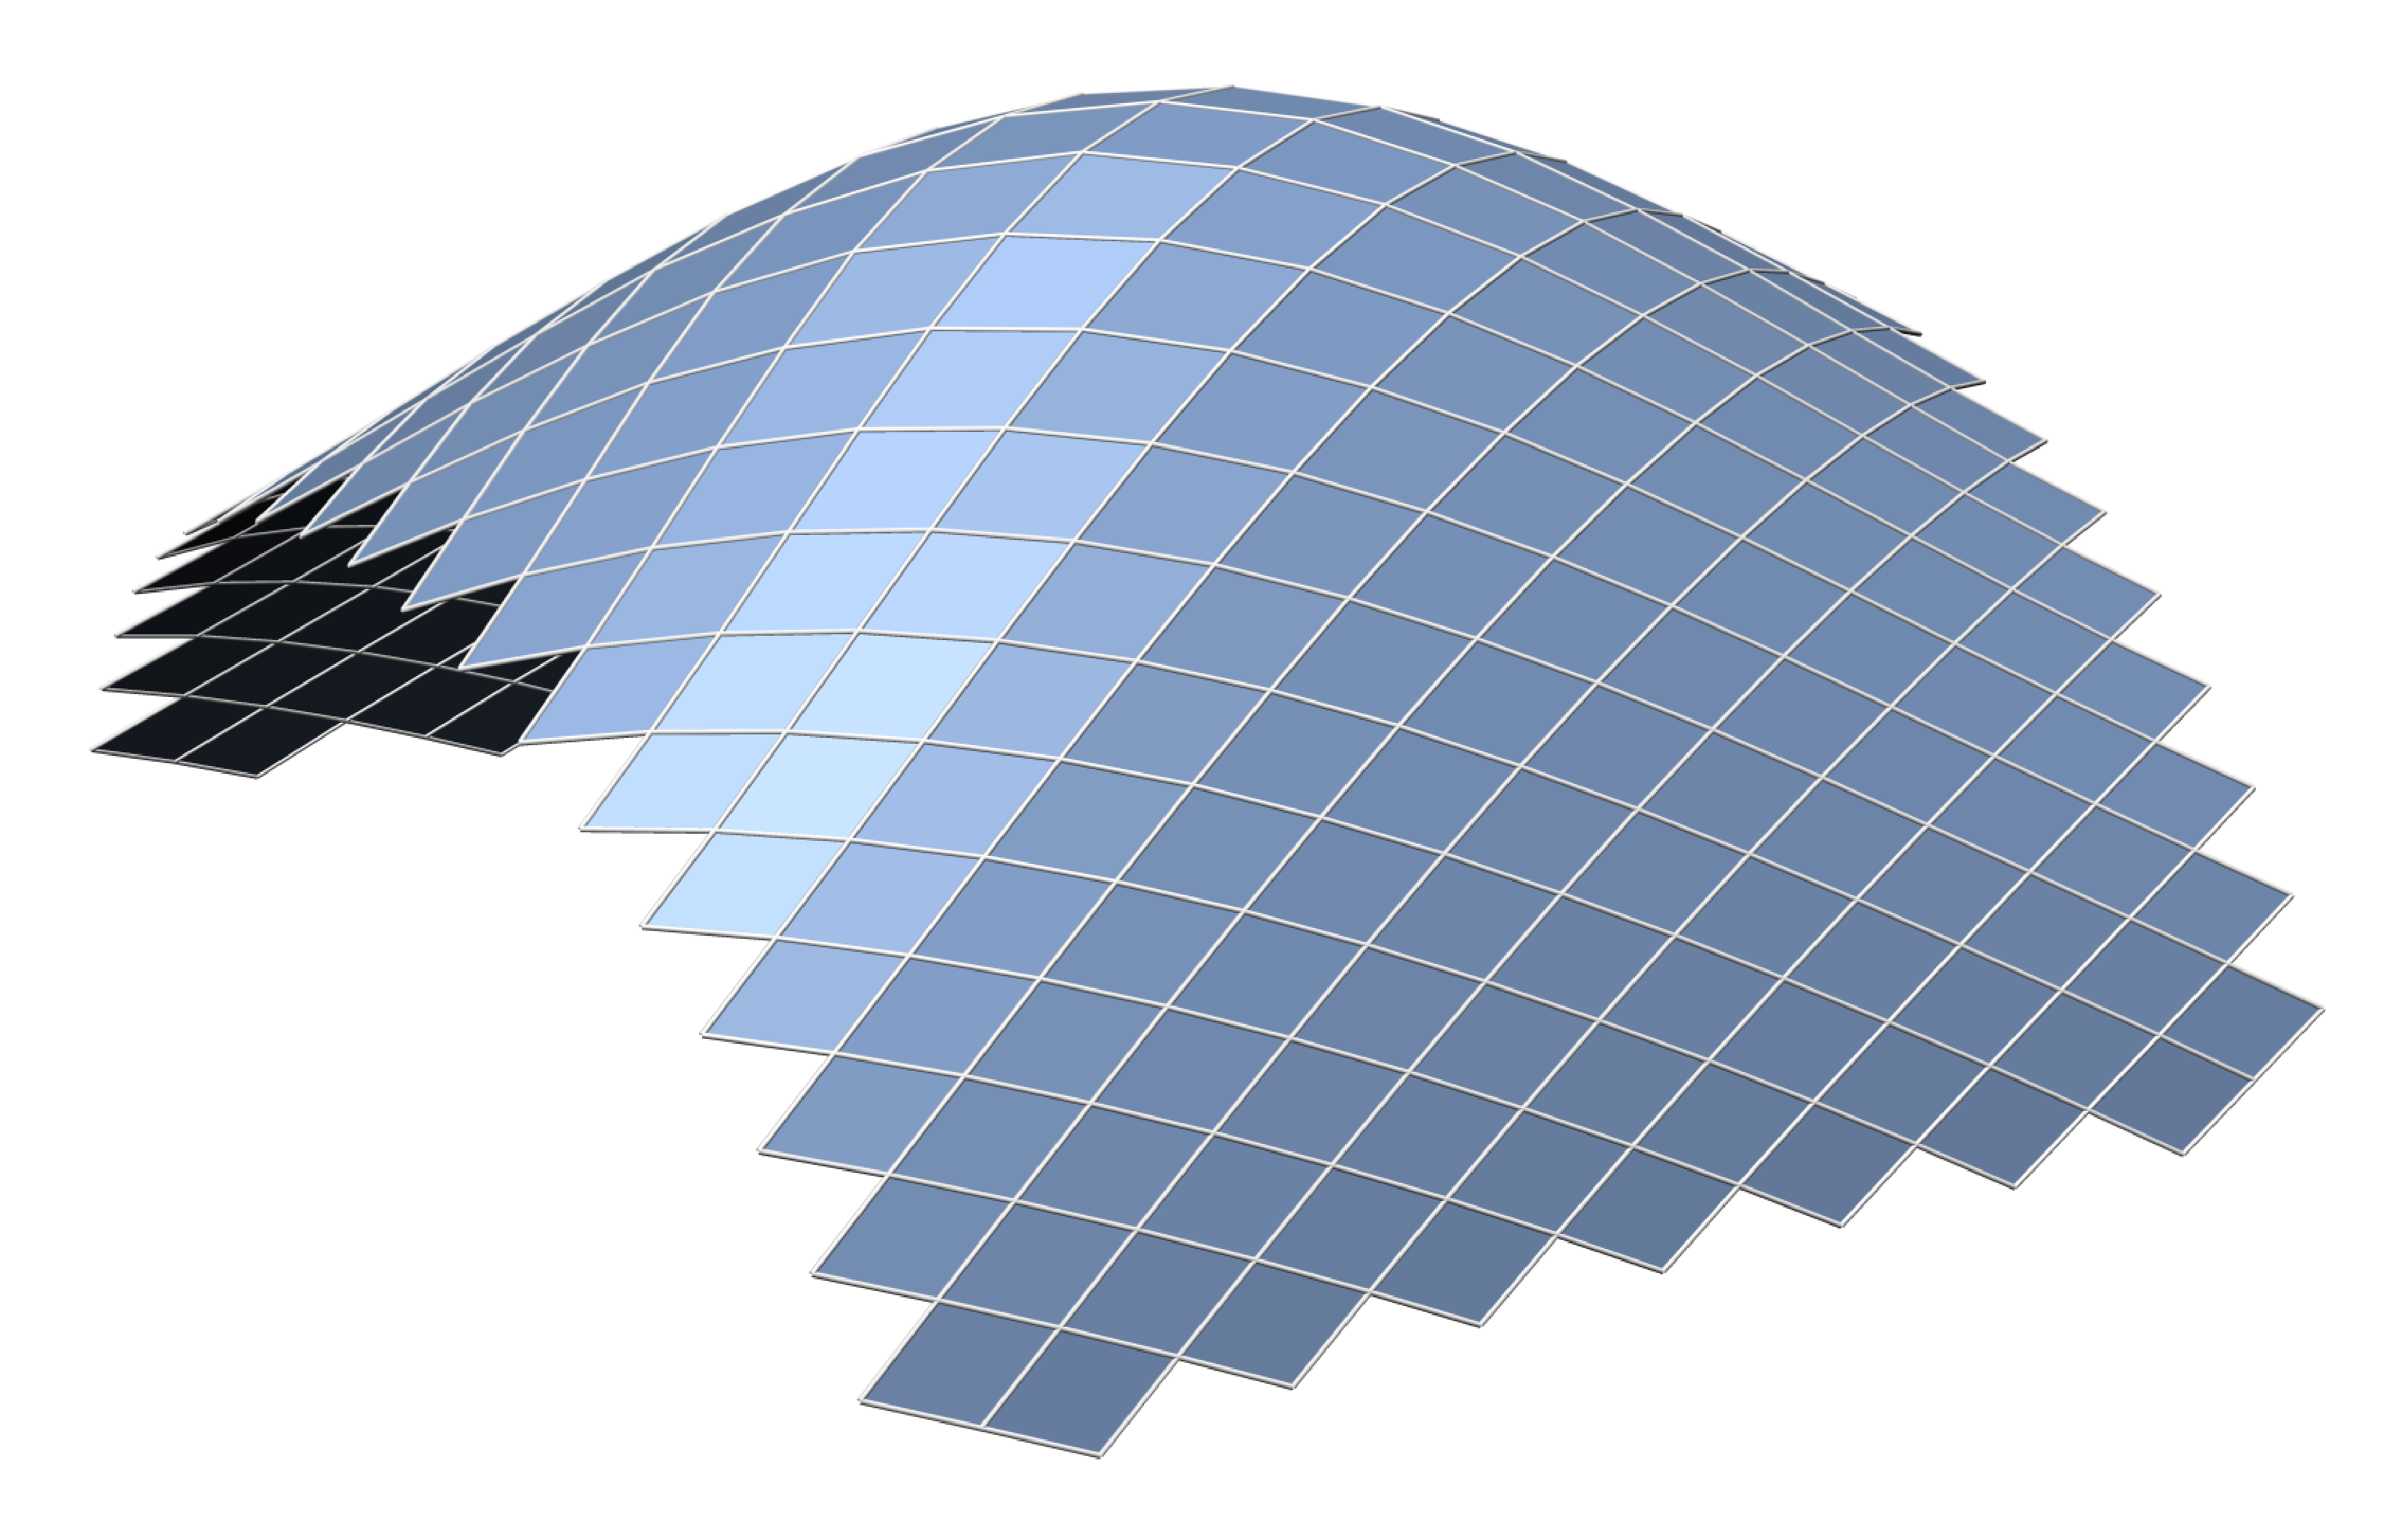
\includegraphics[width=0.33\linewidth]{image/tscheby/init60_mesh.pdf}
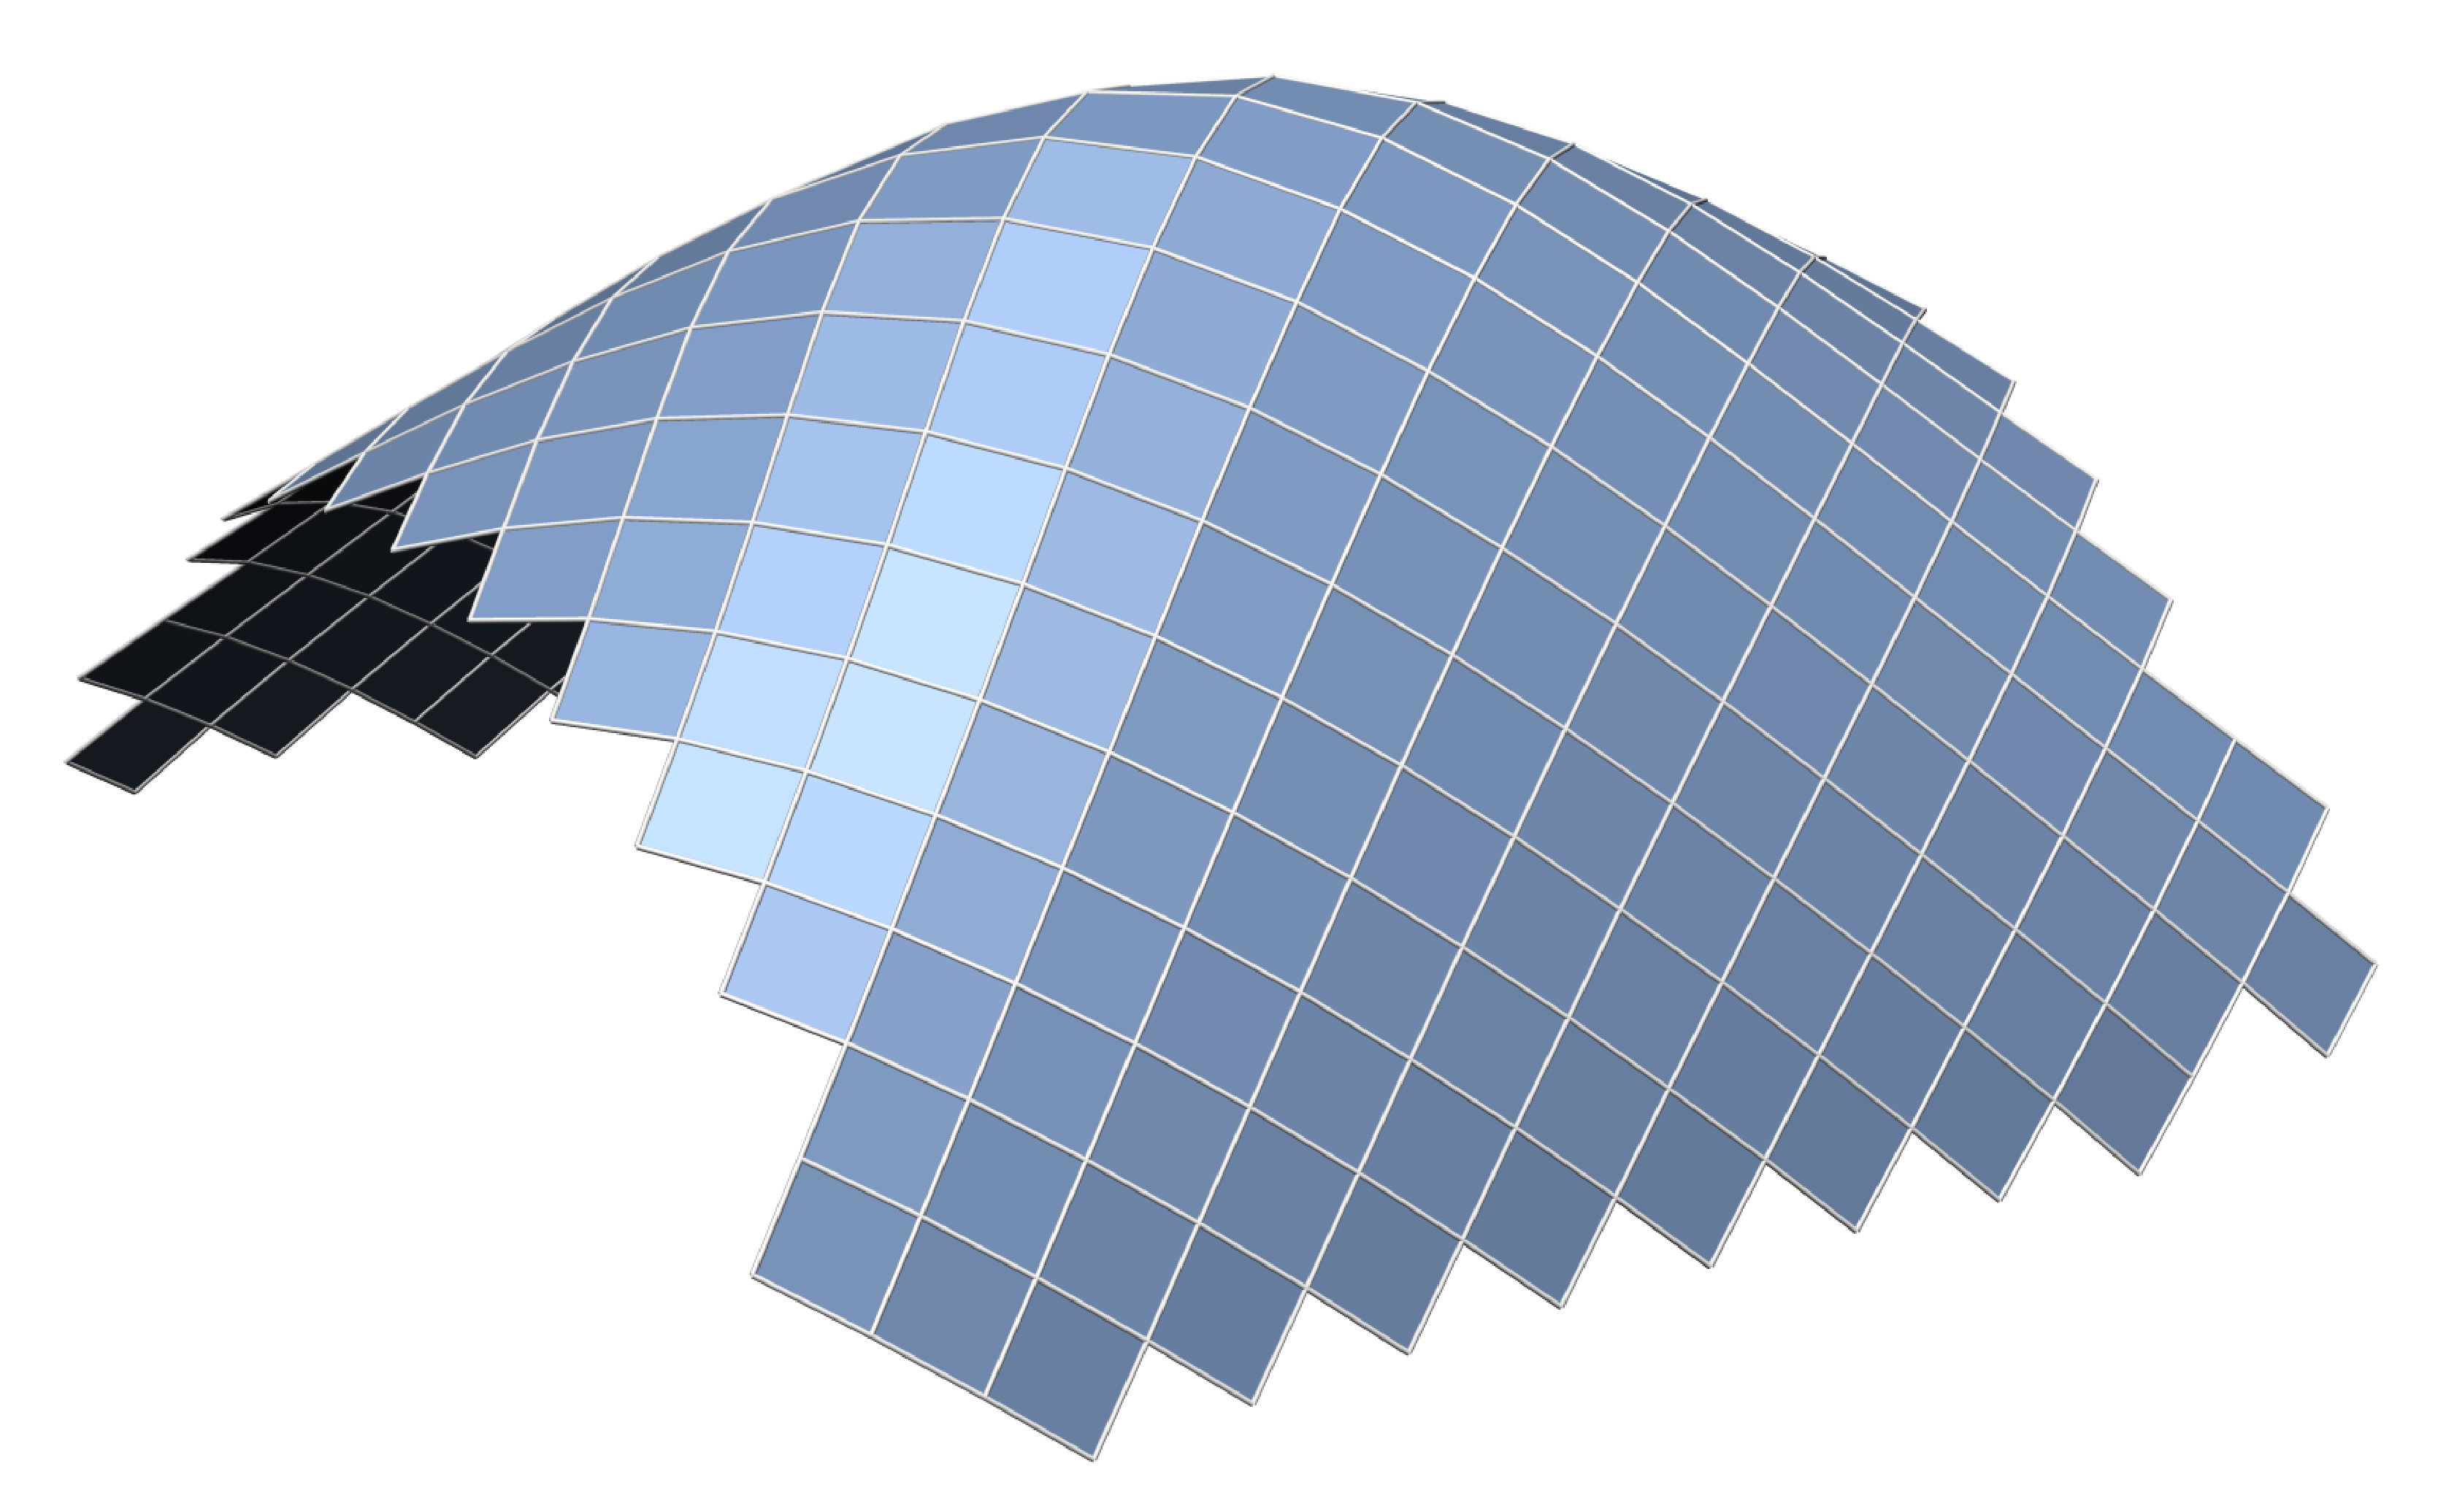
\includegraphics[width=0.33\linewidth]{image/tscheby/init90_mesh.pdf}
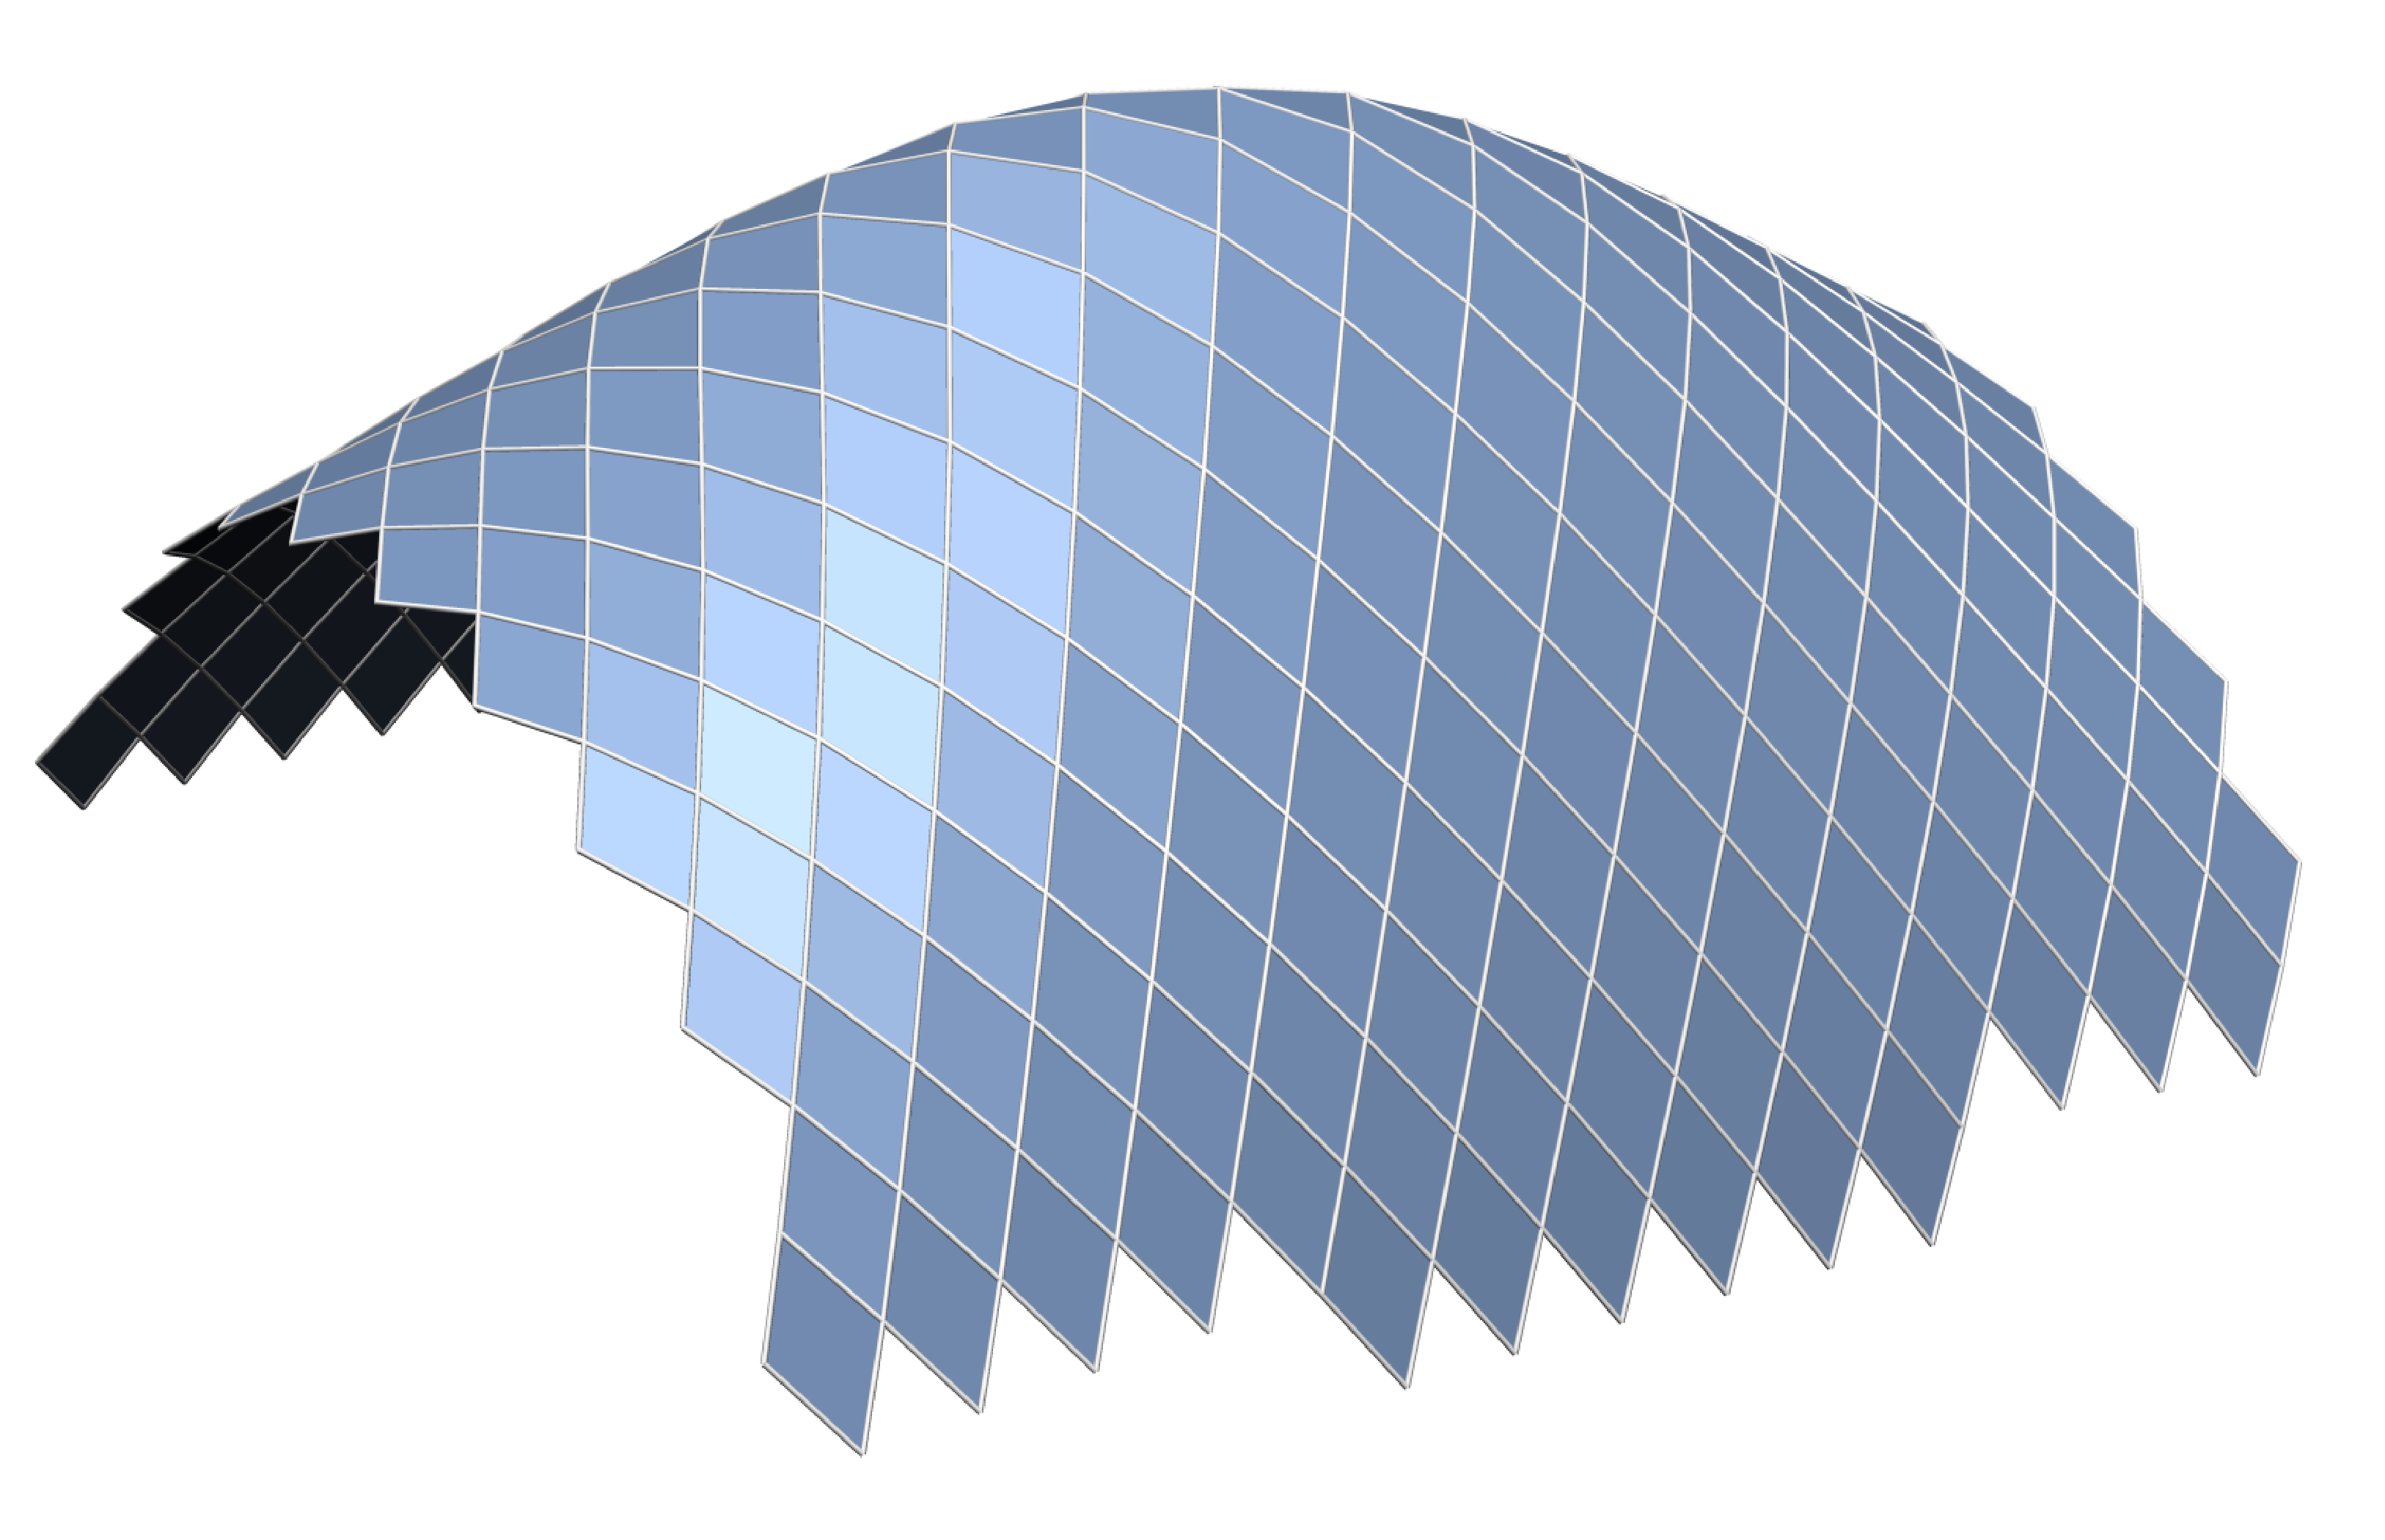
\includegraphics[width=0.33\linewidth]{image/tscheby/init120_mesh.pdf}
}
\caption{Different initialization shear angles for a conformal re-mesh. $30^\circ$ left, $0^\circ$ middle, and $-30^\circ$ right.}
\label{fig:initial_grids}
\end{figure}
\subsection{Initialization and parameters}
The energy $E(M)$ is in general non-convex. That means there can be many local optima, and the solution found by some gradient descent depends on the initialization. We propose to use a conformal re-mesh of the reference surface as initialization. The conformality of the parameterization gives us control over the angles between edges of the quadrilaterals. We can introduce shear to the parameterization and modify this angle globally. By this we start with meshes that have almost constant edge angle, see Figure~\ref{fig:initial_grids}.

\subsection{Implementation}
We use the conformal mapping algorithm by Springborn~\emph{et~al.}~\cite{Springborn2008} to create the
initial mesh. To minimize the energy $E(M)$ we use the non-linear optimization package
PETSc/TAO \cite{petsc-web-page,tao-user-ref} and its java binding 
\cite{jpetsctao-web-page}. We have made good experiences with normalizing the
 energies to have gradient length one before optimization. Then we start with all
$\lambda$s equal to one and modify them on the way if needed. If one encounters
degenerate configurations during optimization one can drop the length energy term for 
a few iterations.

\section{Case studies regular gridshells}

\subsection{The sphere}
A simple test of our method is the meshing of a part of a sphere. We will compare our results with a reference mesh that we obtain from a special smooth parameterization of the sphere. Namely there is a smooth parameterization of the sphere that has the property that the lengths of partial derivatives are constant throughout the surface. That means that for small discretization steps we can produce meshes with equal edge lengths from such a parameterization. The formula for this unit sphere can be found in the work of Voss~\cite{Voss1881}:
\begin{eqnarray*}
	x(u,v)&=&\sn(u+v, k)\cdot \cos(k\cdot (u-v))\\
	y(u,v)&=&\sn(u+v, k)\cdot \sin(k\cdot (u-v))\\
	z(u,v)&=&\cn(u+v, k).
\end{eqnarray*}
Here $\sn$ and $\cn$ are the Jacobi elliptic functions with modulus $k$. For different $k\in ]0,1[$ we get spheres with equal edges lengths and different shapes of parameter curves (see Fig.~\ref{fig:spheres}).

\begin{figure}
\centering
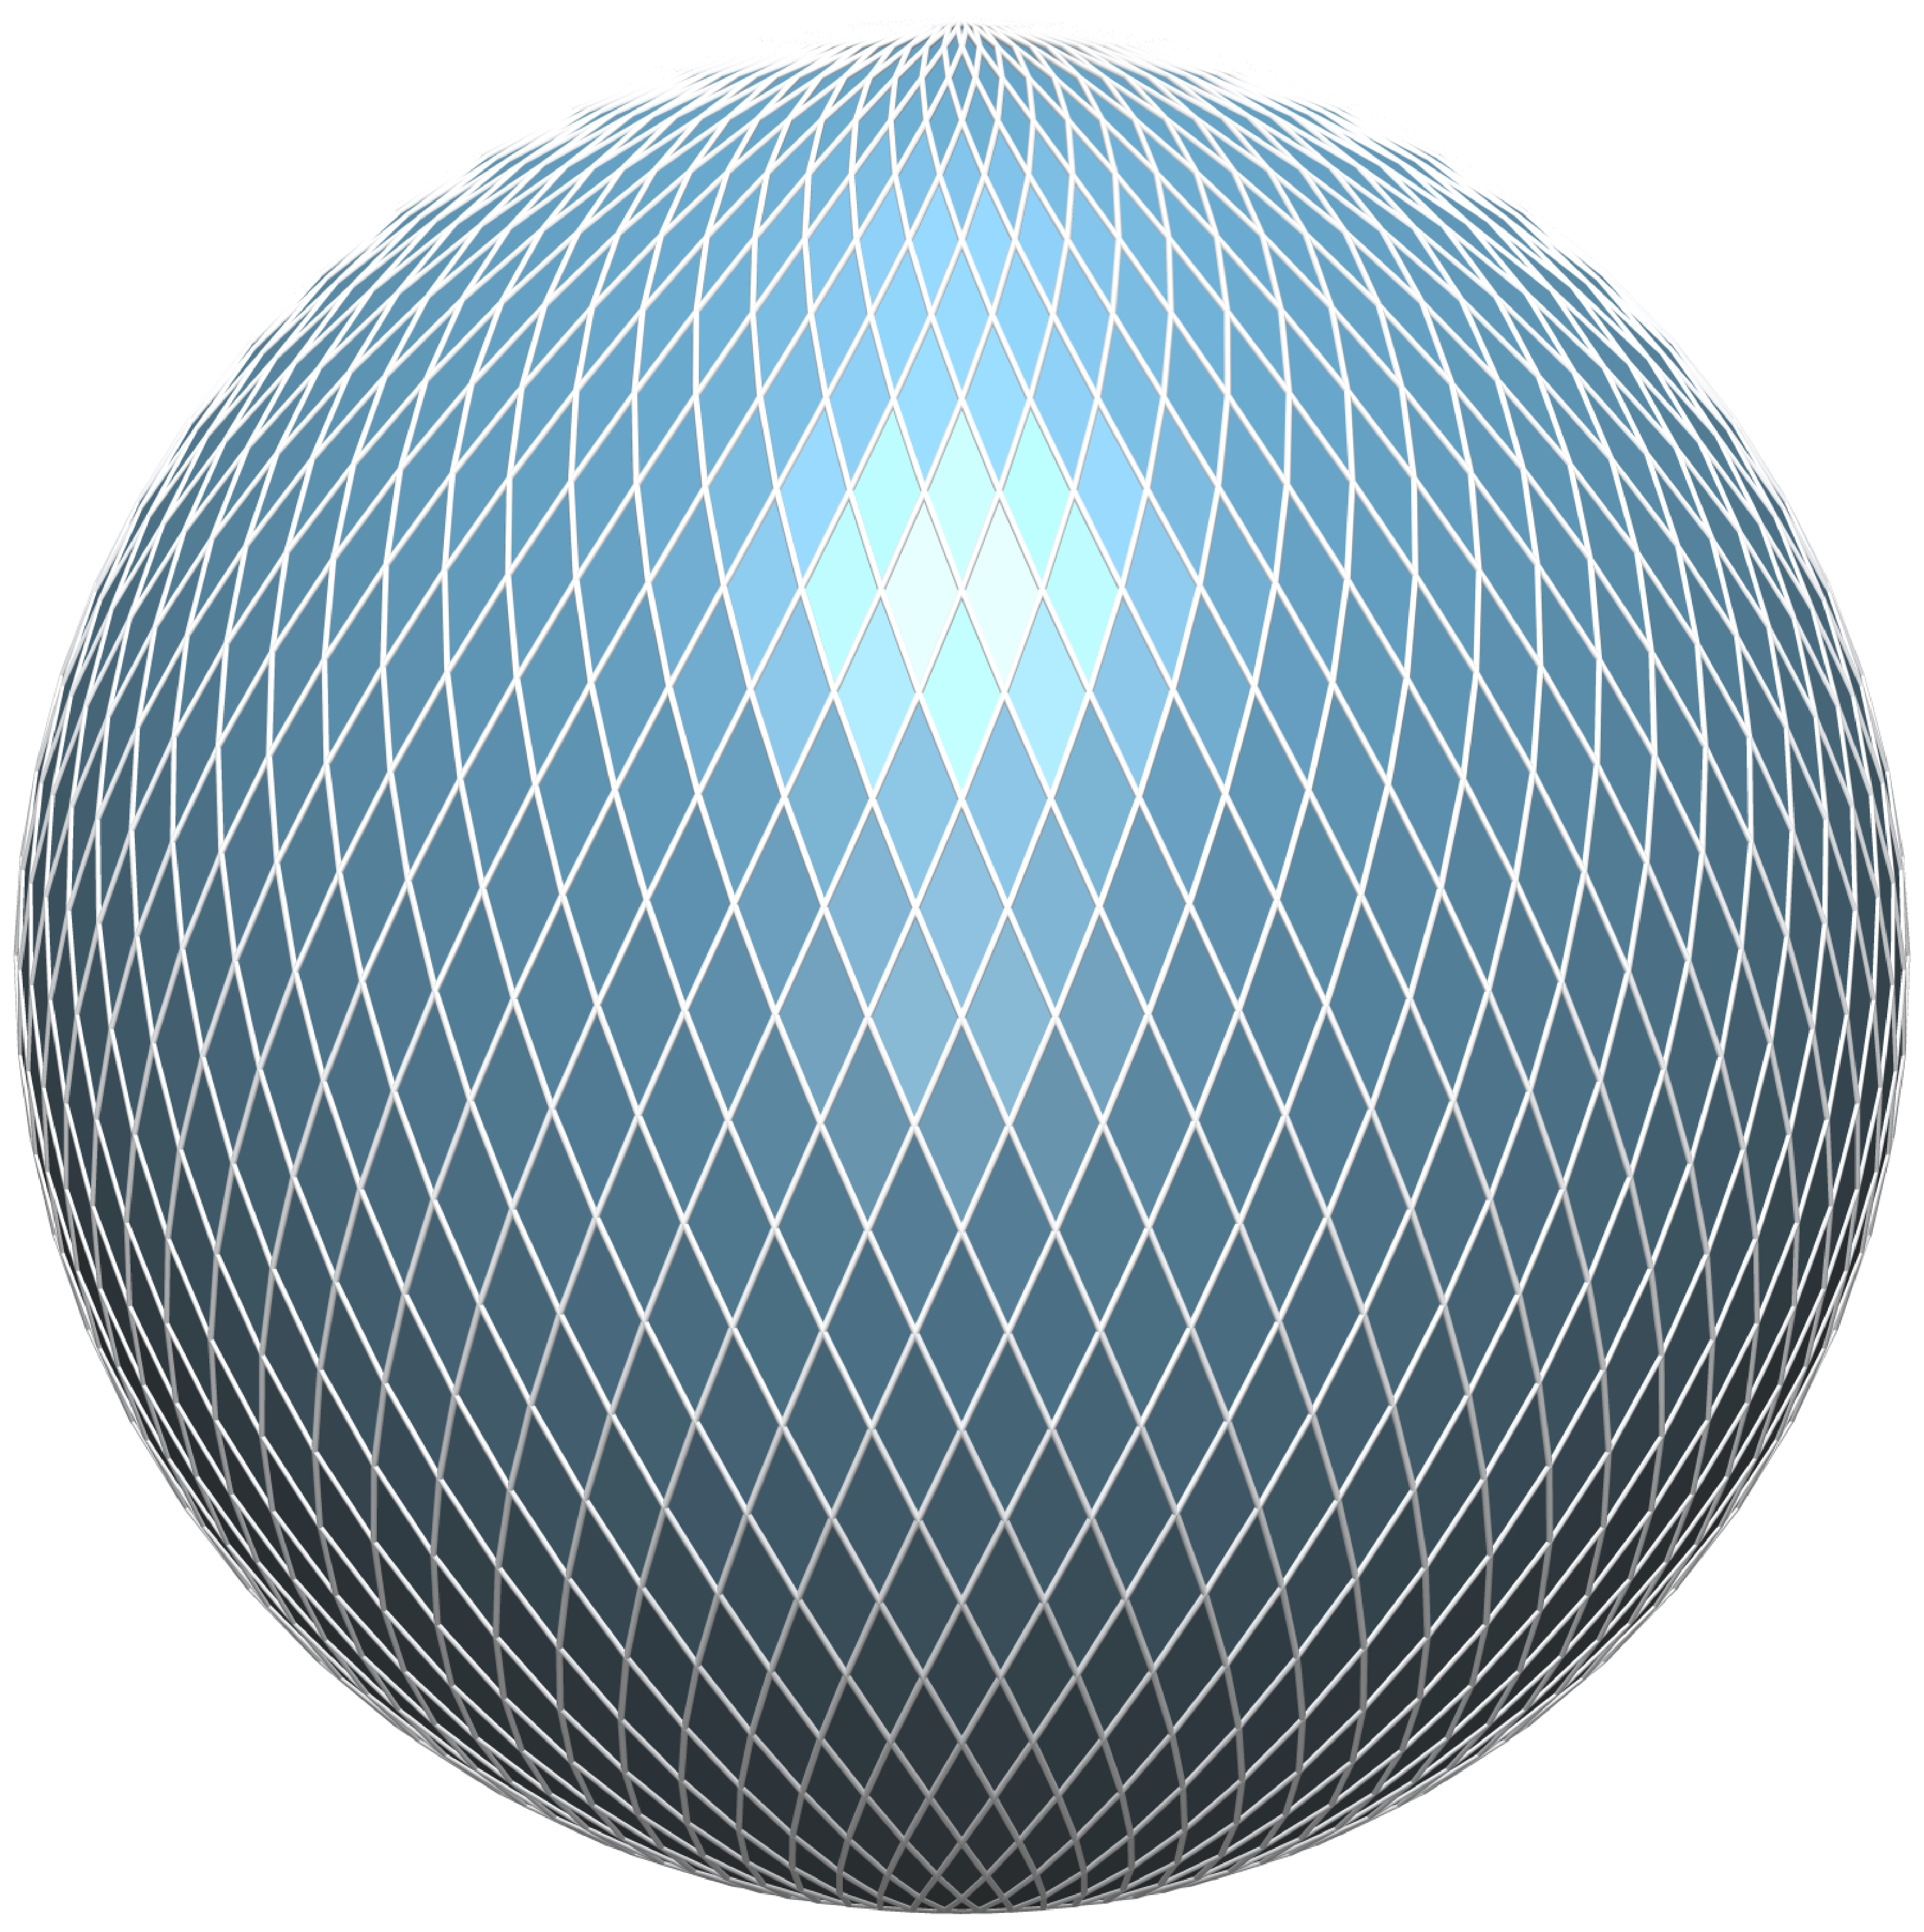
\includegraphics[width=0.32\linewidth]{images/spheres/k0_4_new.pdf}
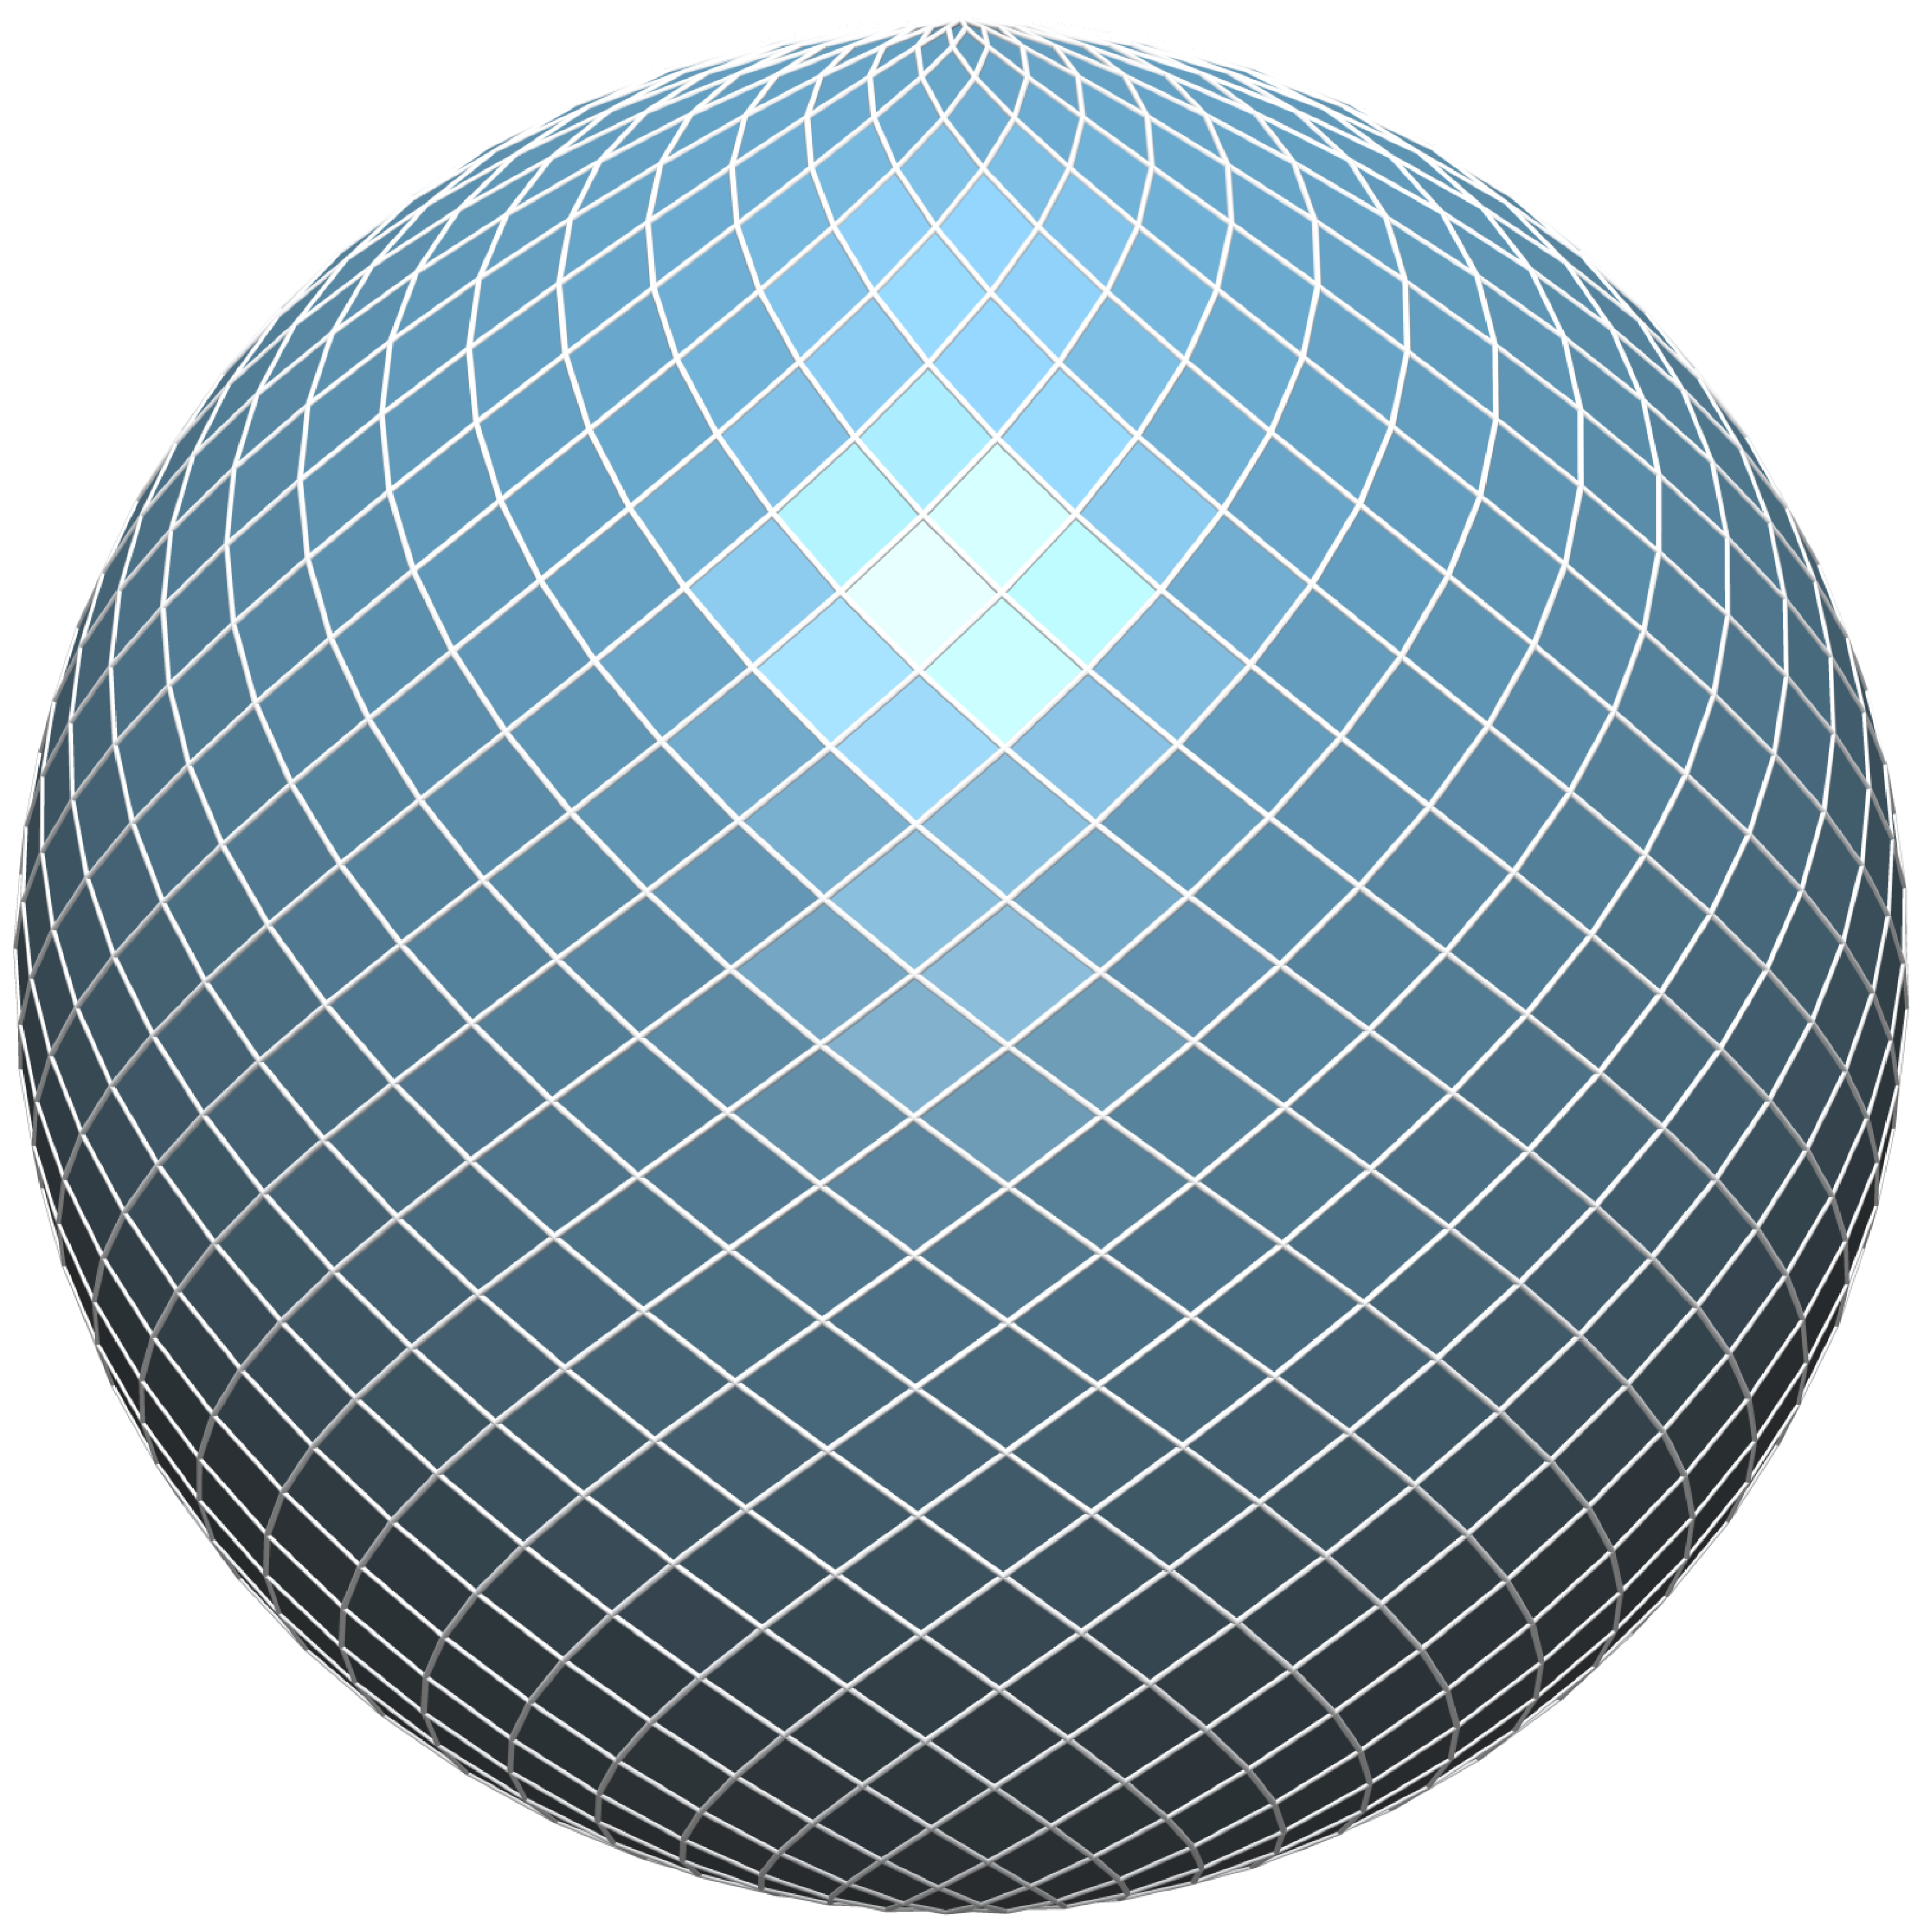
\includegraphics[width=0.32\linewidth]{images/spheres/k0_8_new.pdf}
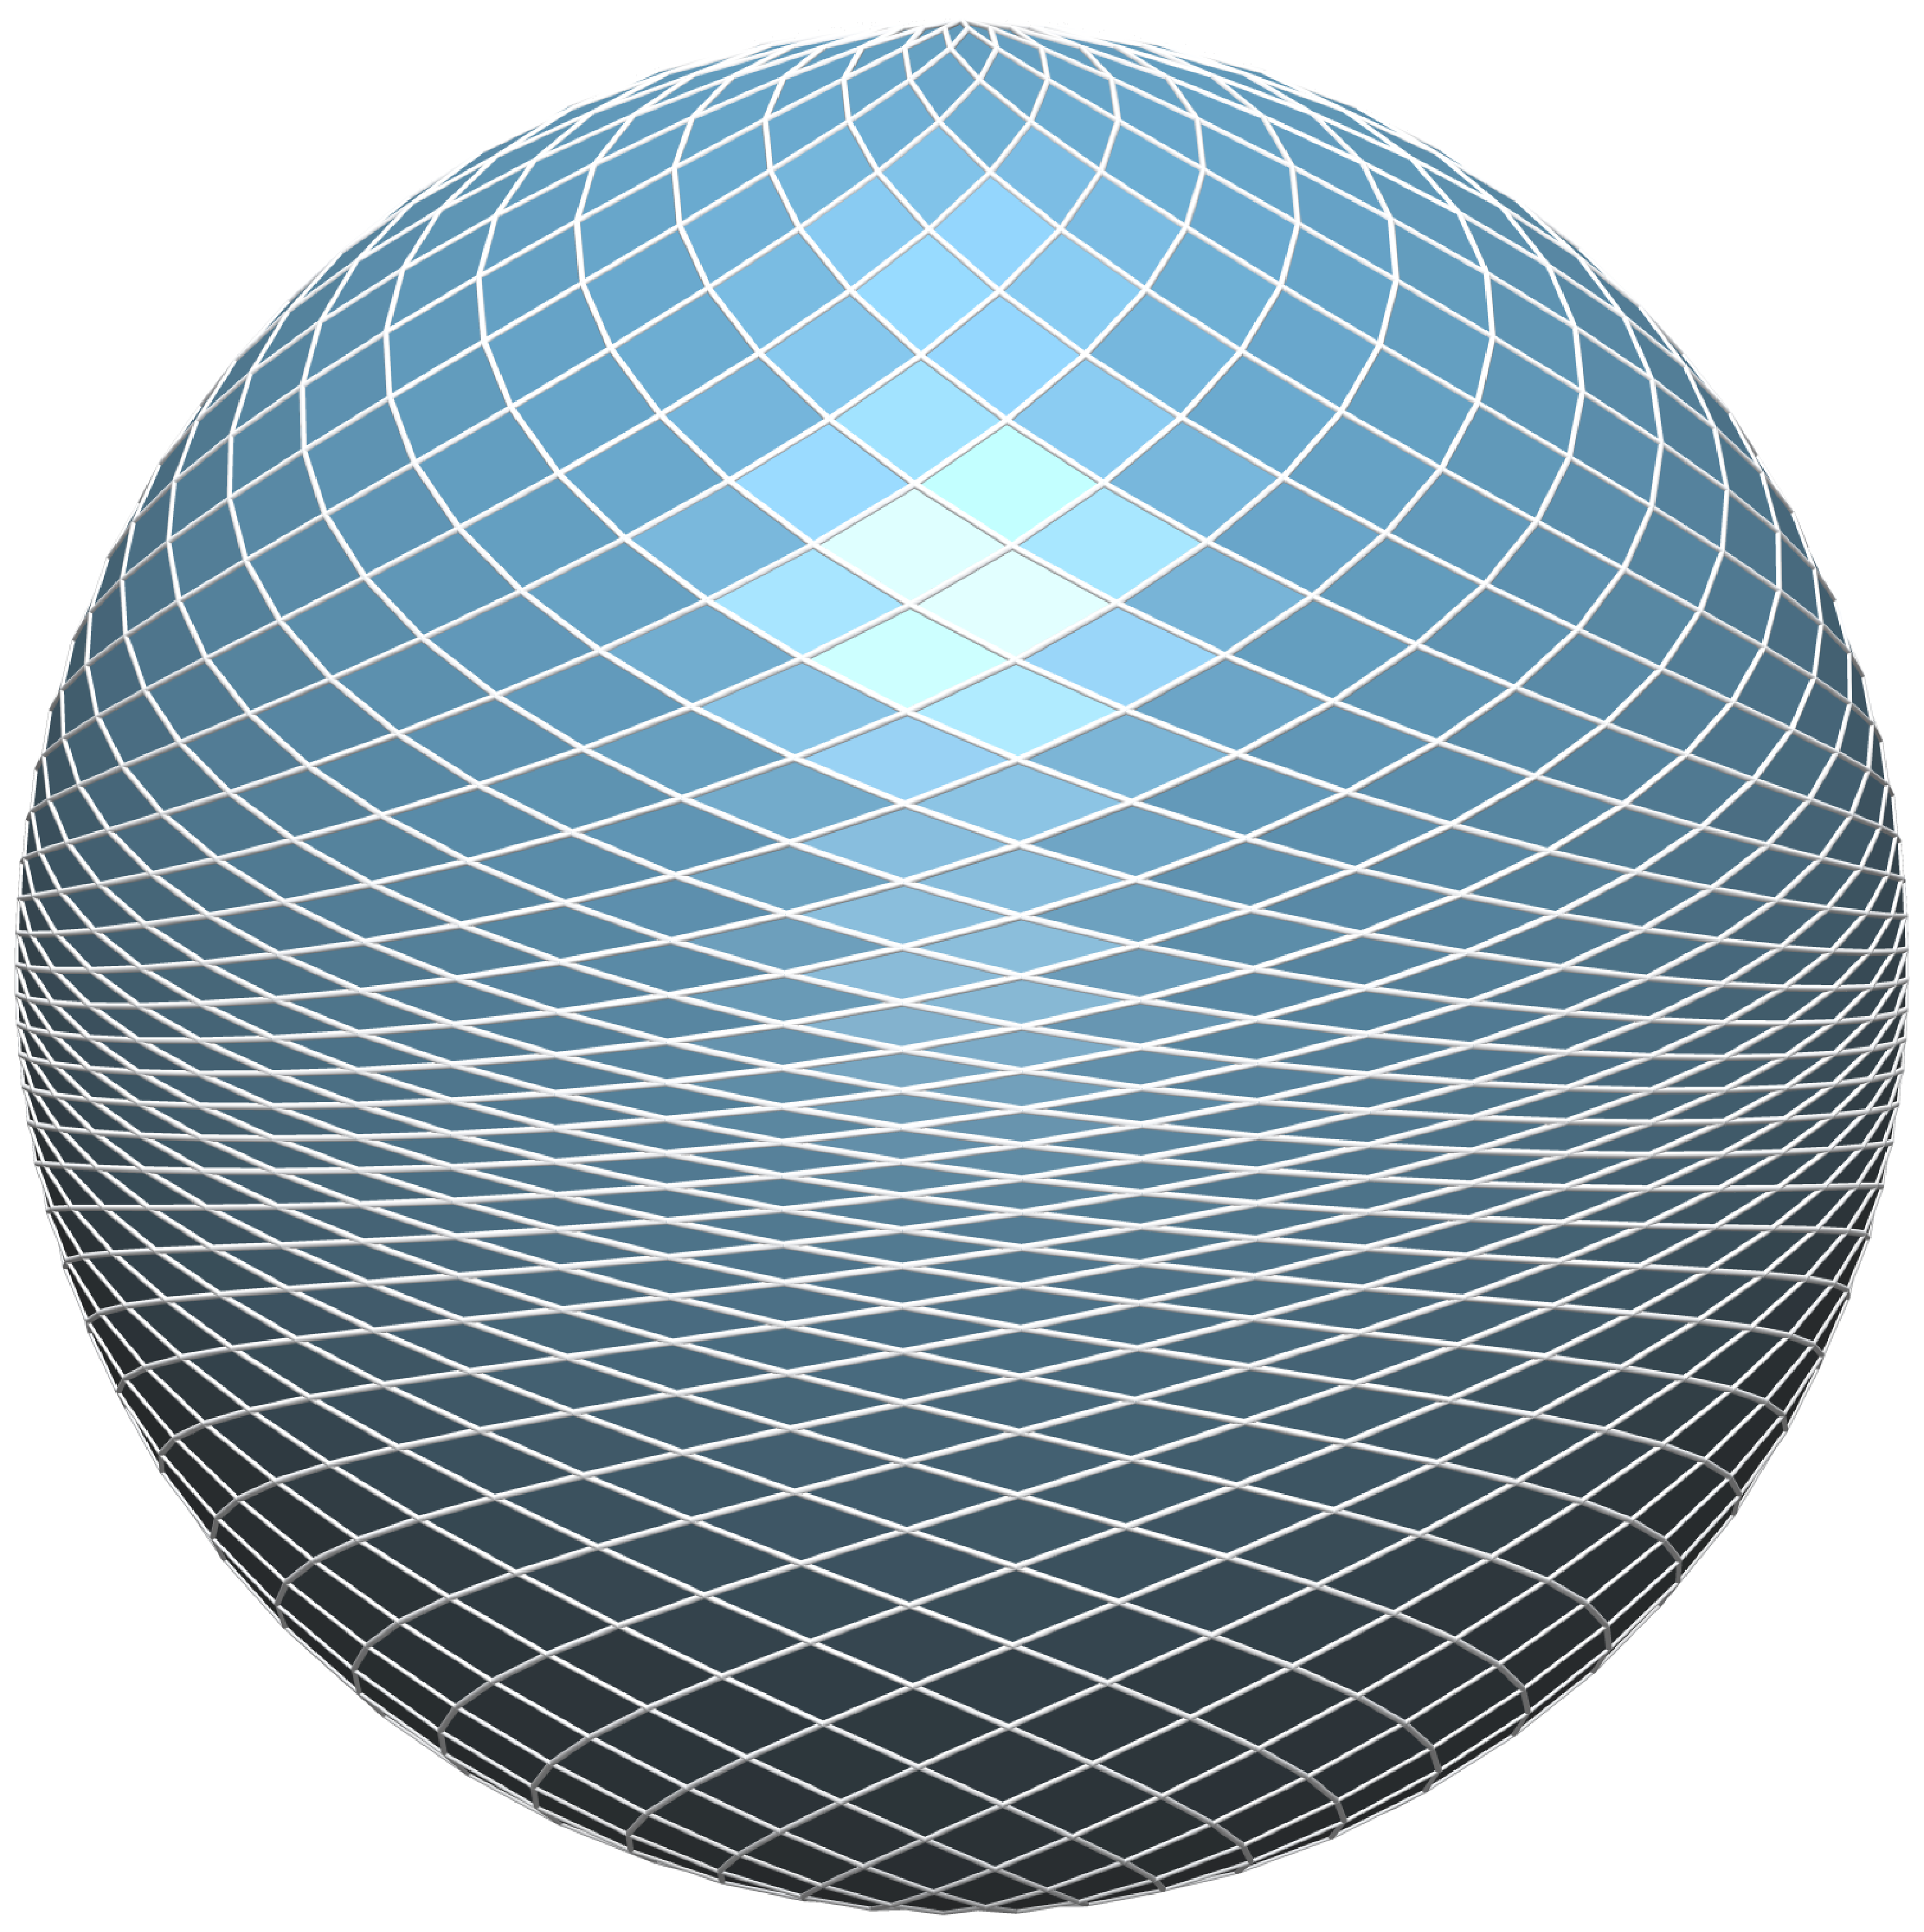
\includegraphics[width=0.32\linewidth]{images/spheres/k0_99_new.pdf}
\caption{Explicitly parameterized spheres with equal edges length $l=0.11$. The parameter $k$ is equal to $0.4$ (left), $0.8$ (middle), and $0.99$ (right).}
\label{fig:spheres}
\end{figure}

We measure qualitative curvature of these curves like in our energy $E_{\textrm{\scriptsize{cur}}}$ as $(\pi - \angle(e,\tilde e))^2$. Where $e$ and $\tilde e$ are opposite edges at a vertex of the quad mesh. The curvature mean of the parameter curves is decreasing for $k$ approaching zero, see Figure~\ref{fig:curvature_plot}.
\begin{figure}
\centering
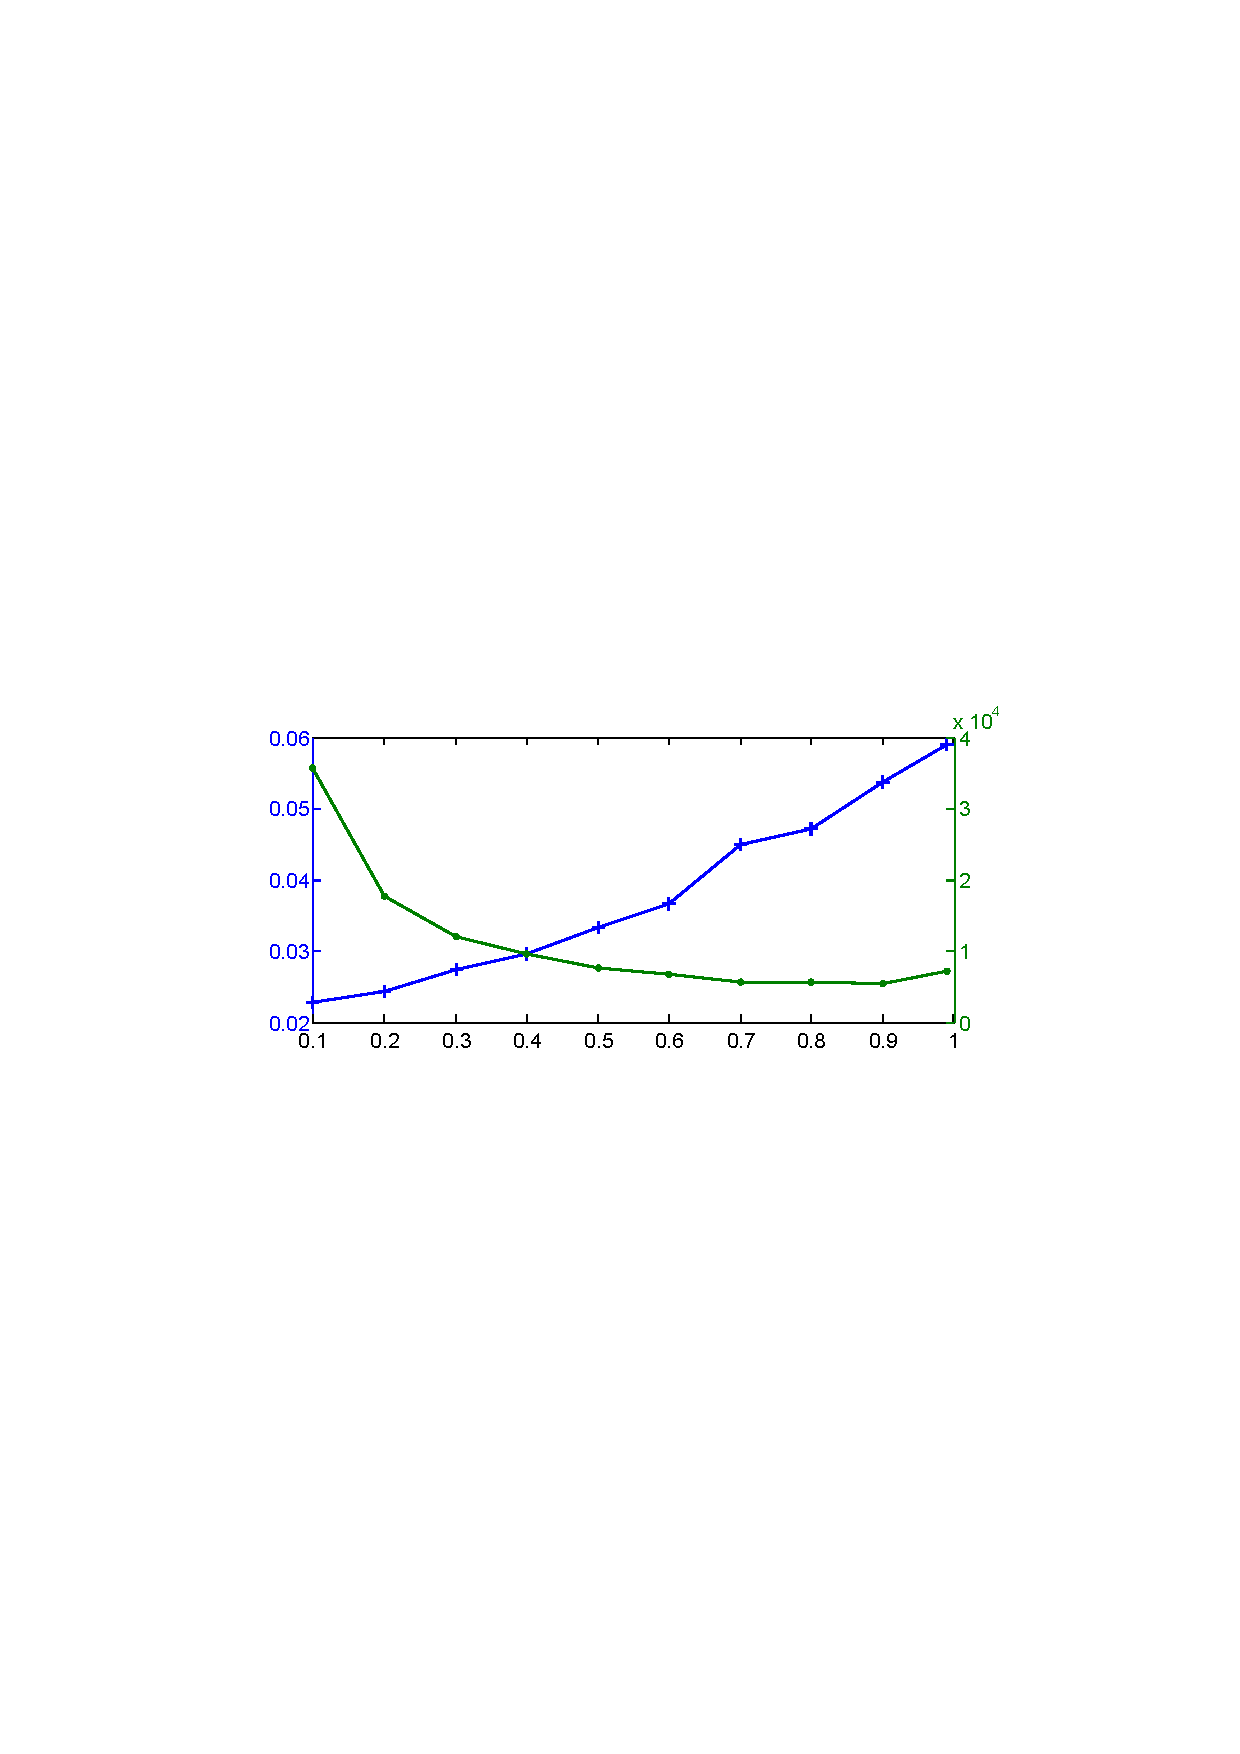
\includegraphics[width=0.7\linewidth]{images/spheres/curvature2_embedded.pdf}
\caption{The mean value of $(\pi - \angle(e,\tilde e))^2$ (blue) on parameter curves of the explicit sphere parameterization is plotted against the parameter $k$. The green curve indicates the number of edges in the corresponding mesh.}
\label{fig:curvature_plot}
\end{figure}
Using our optimization scheme from the previous section we can reproduce the mesh shapes obtained for different $k$. The initial mesh is here a sheared conformal re-mesh of a part of the unit sphere, see Figure~\ref{fig:spheres_optimized}.
\begin{figure}
\centering
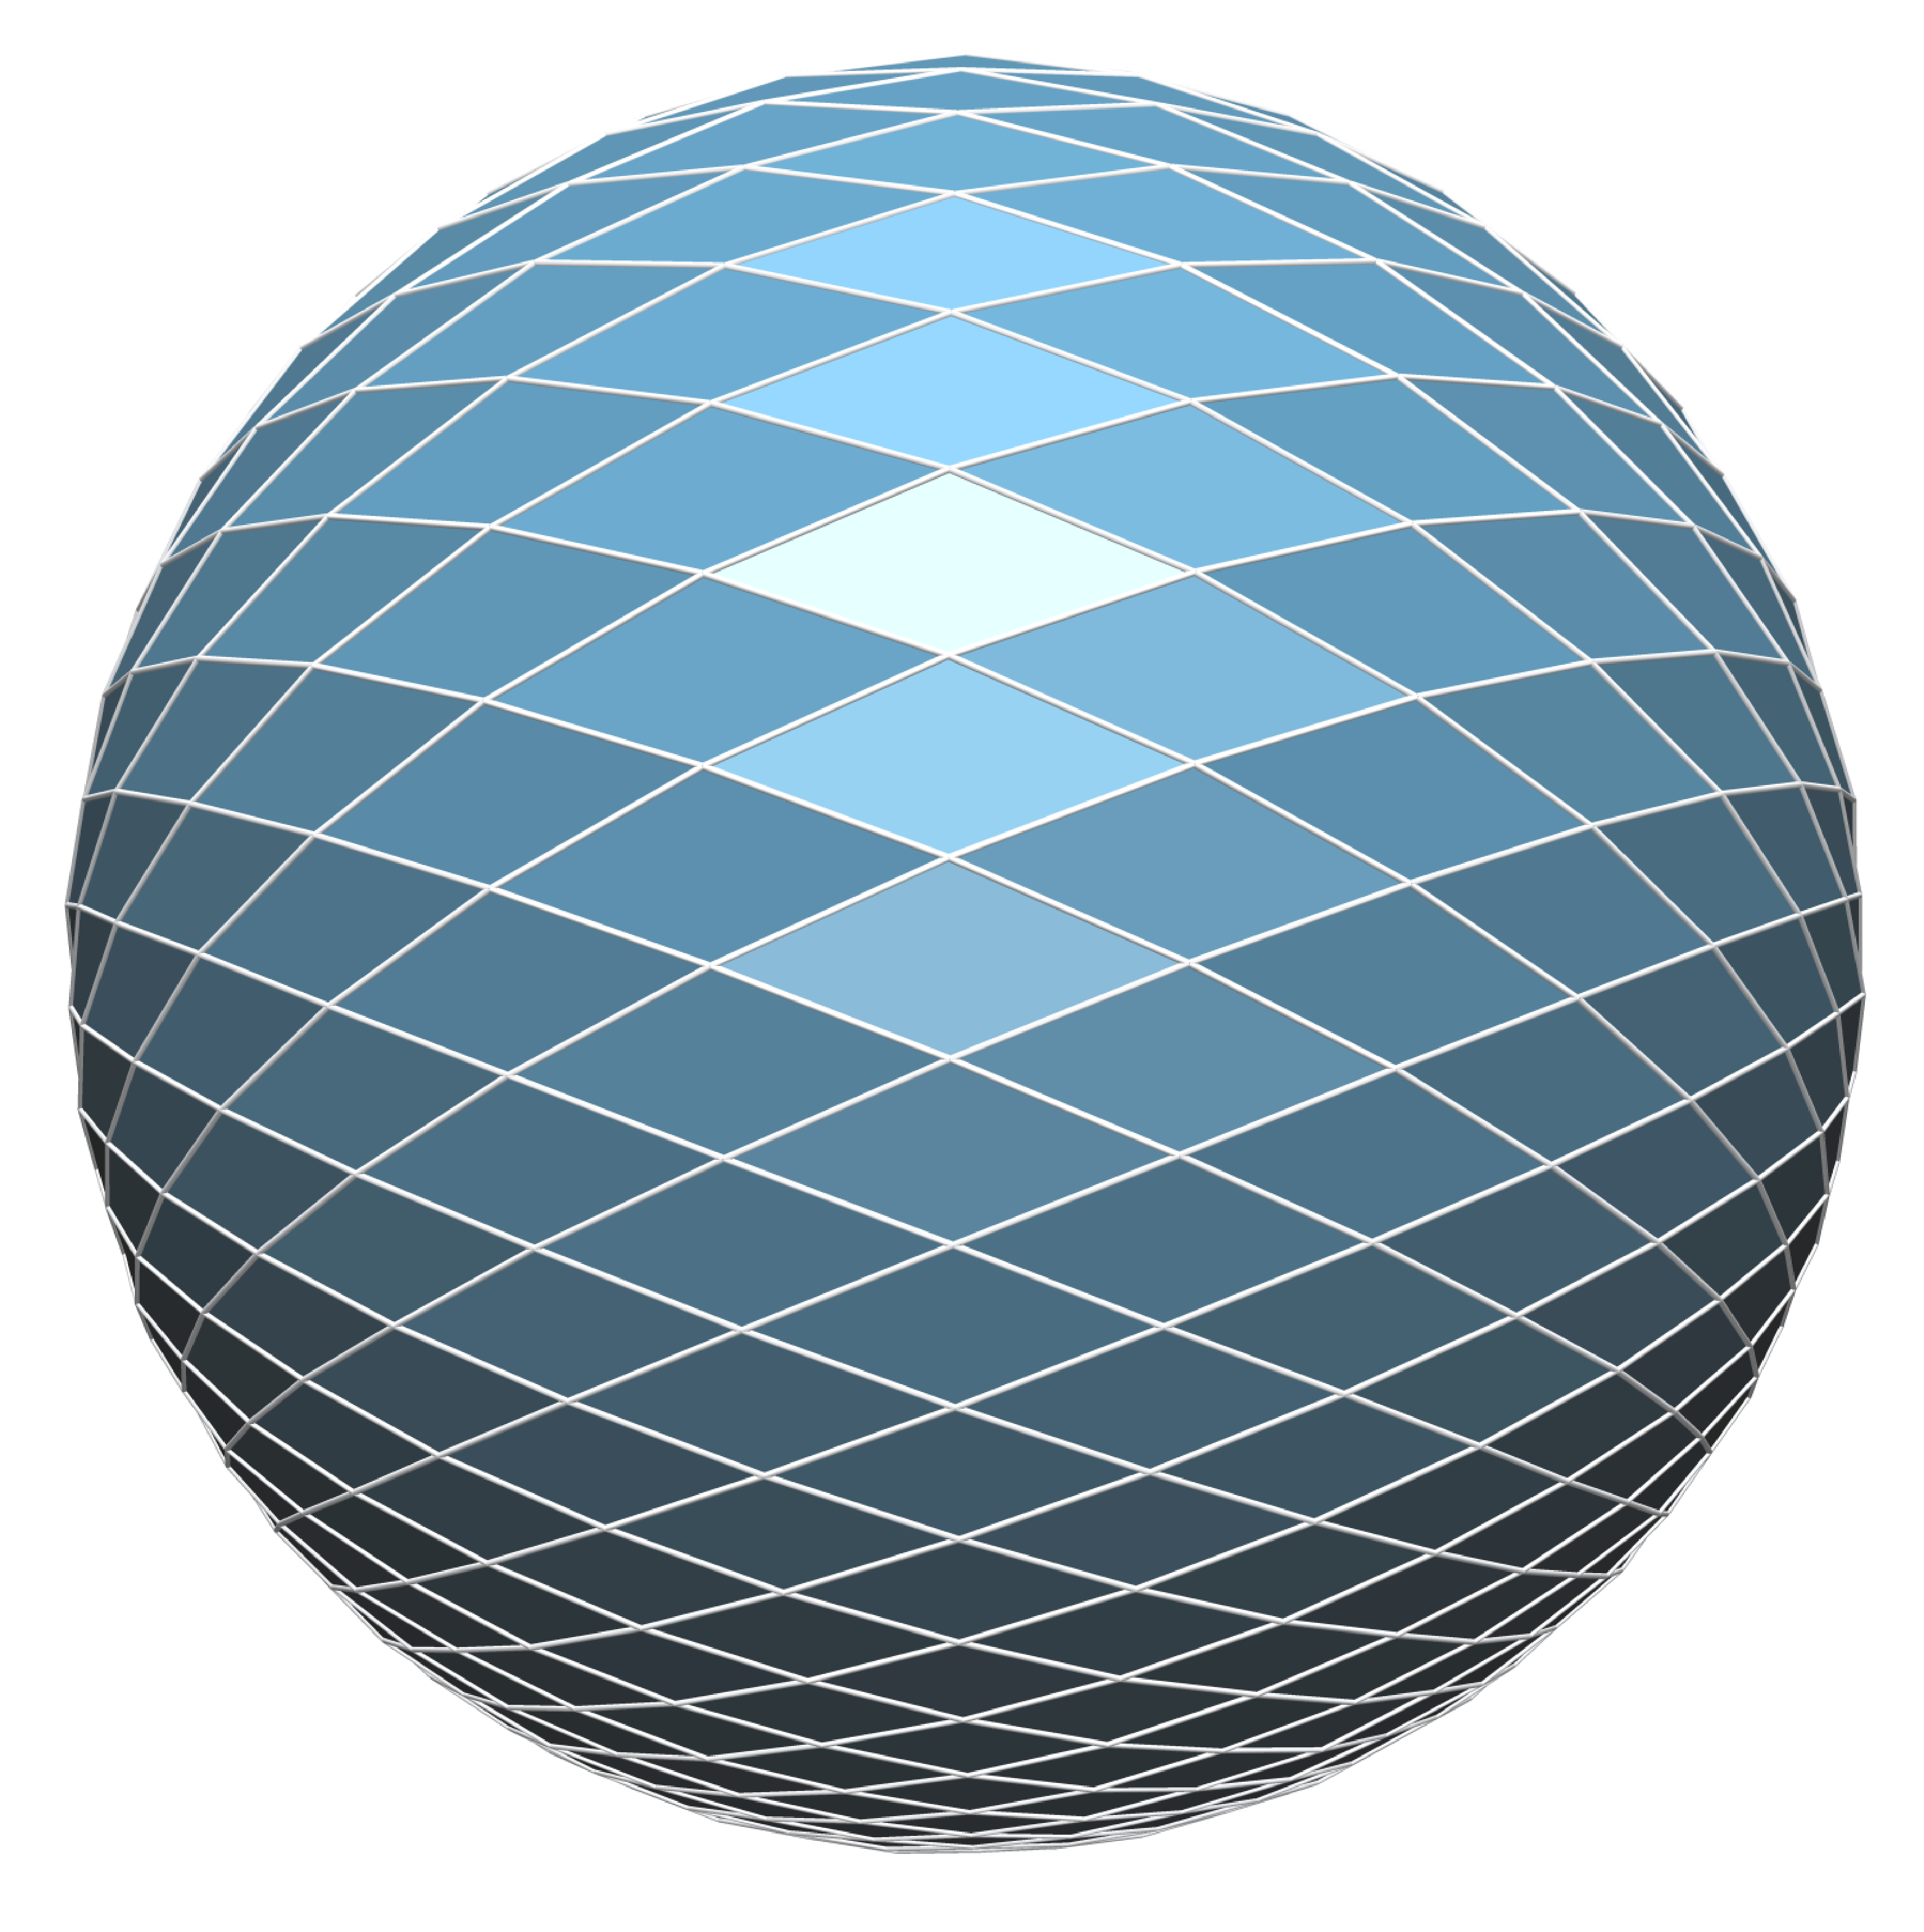
\includegraphics[width=0.32\linewidth]{images/spheres/start45_new.pdf}
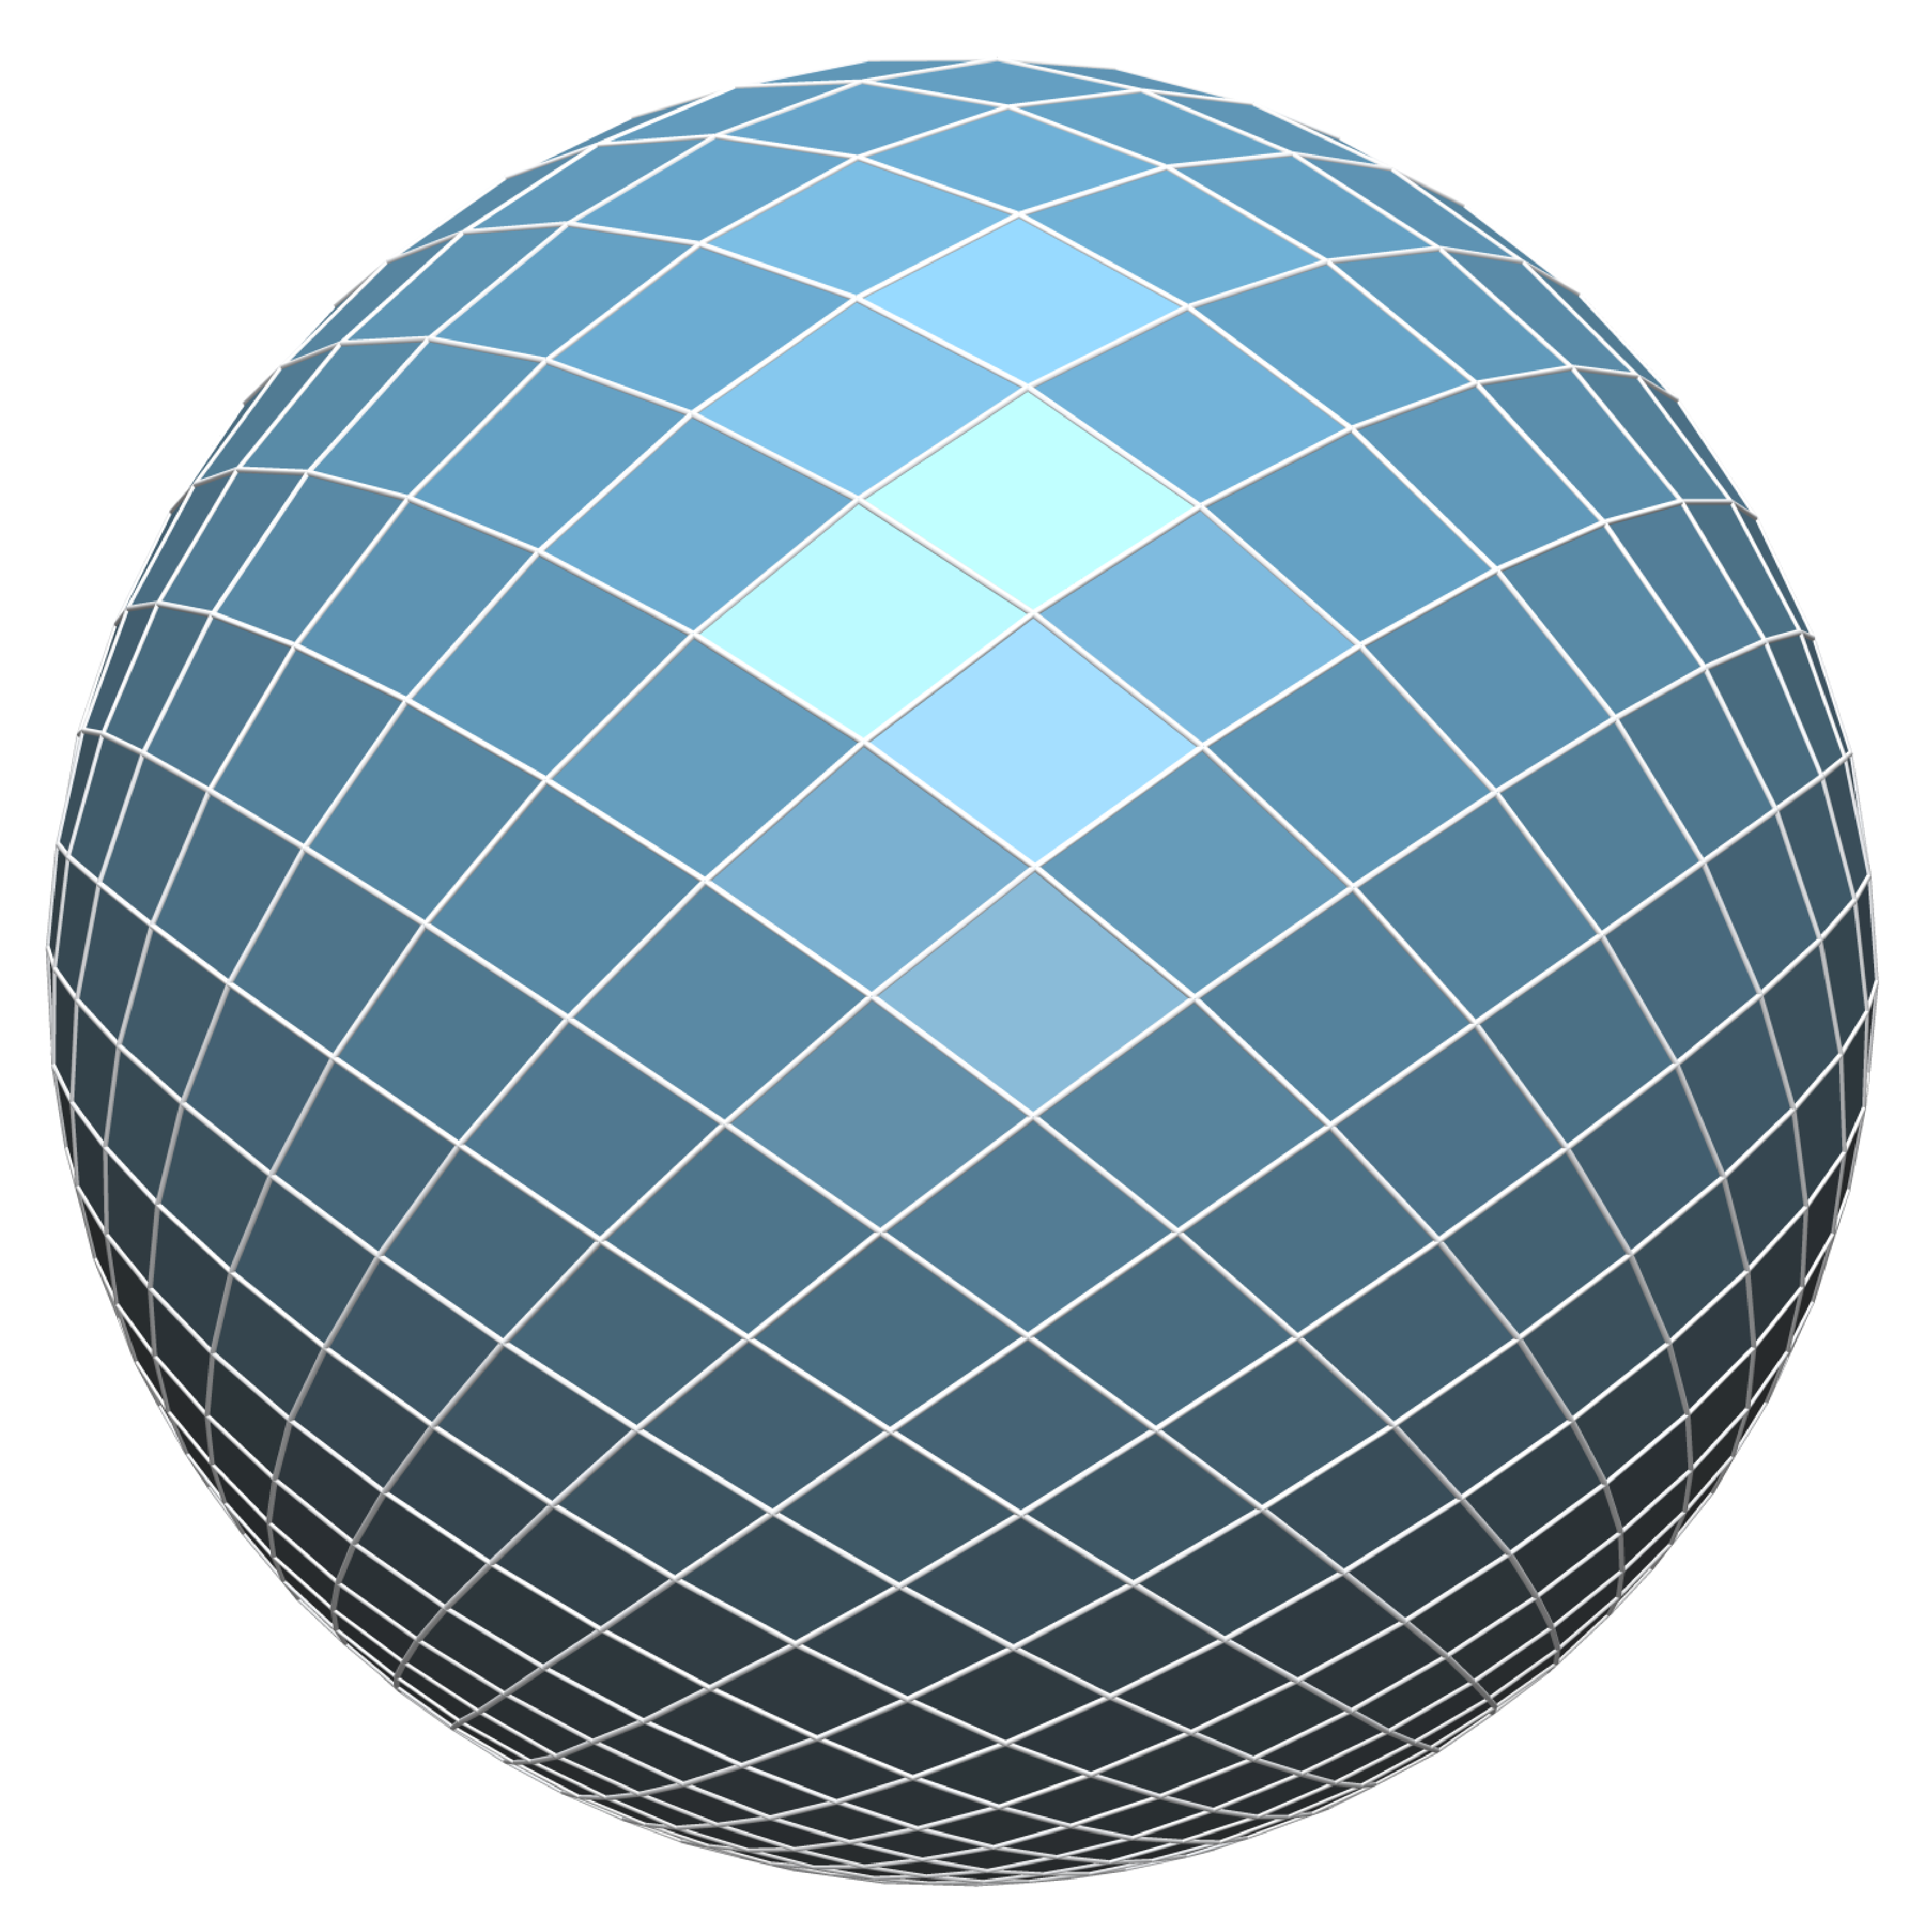
\includegraphics[width=0.32\linewidth]{images/spheres/start15_new.pdf}
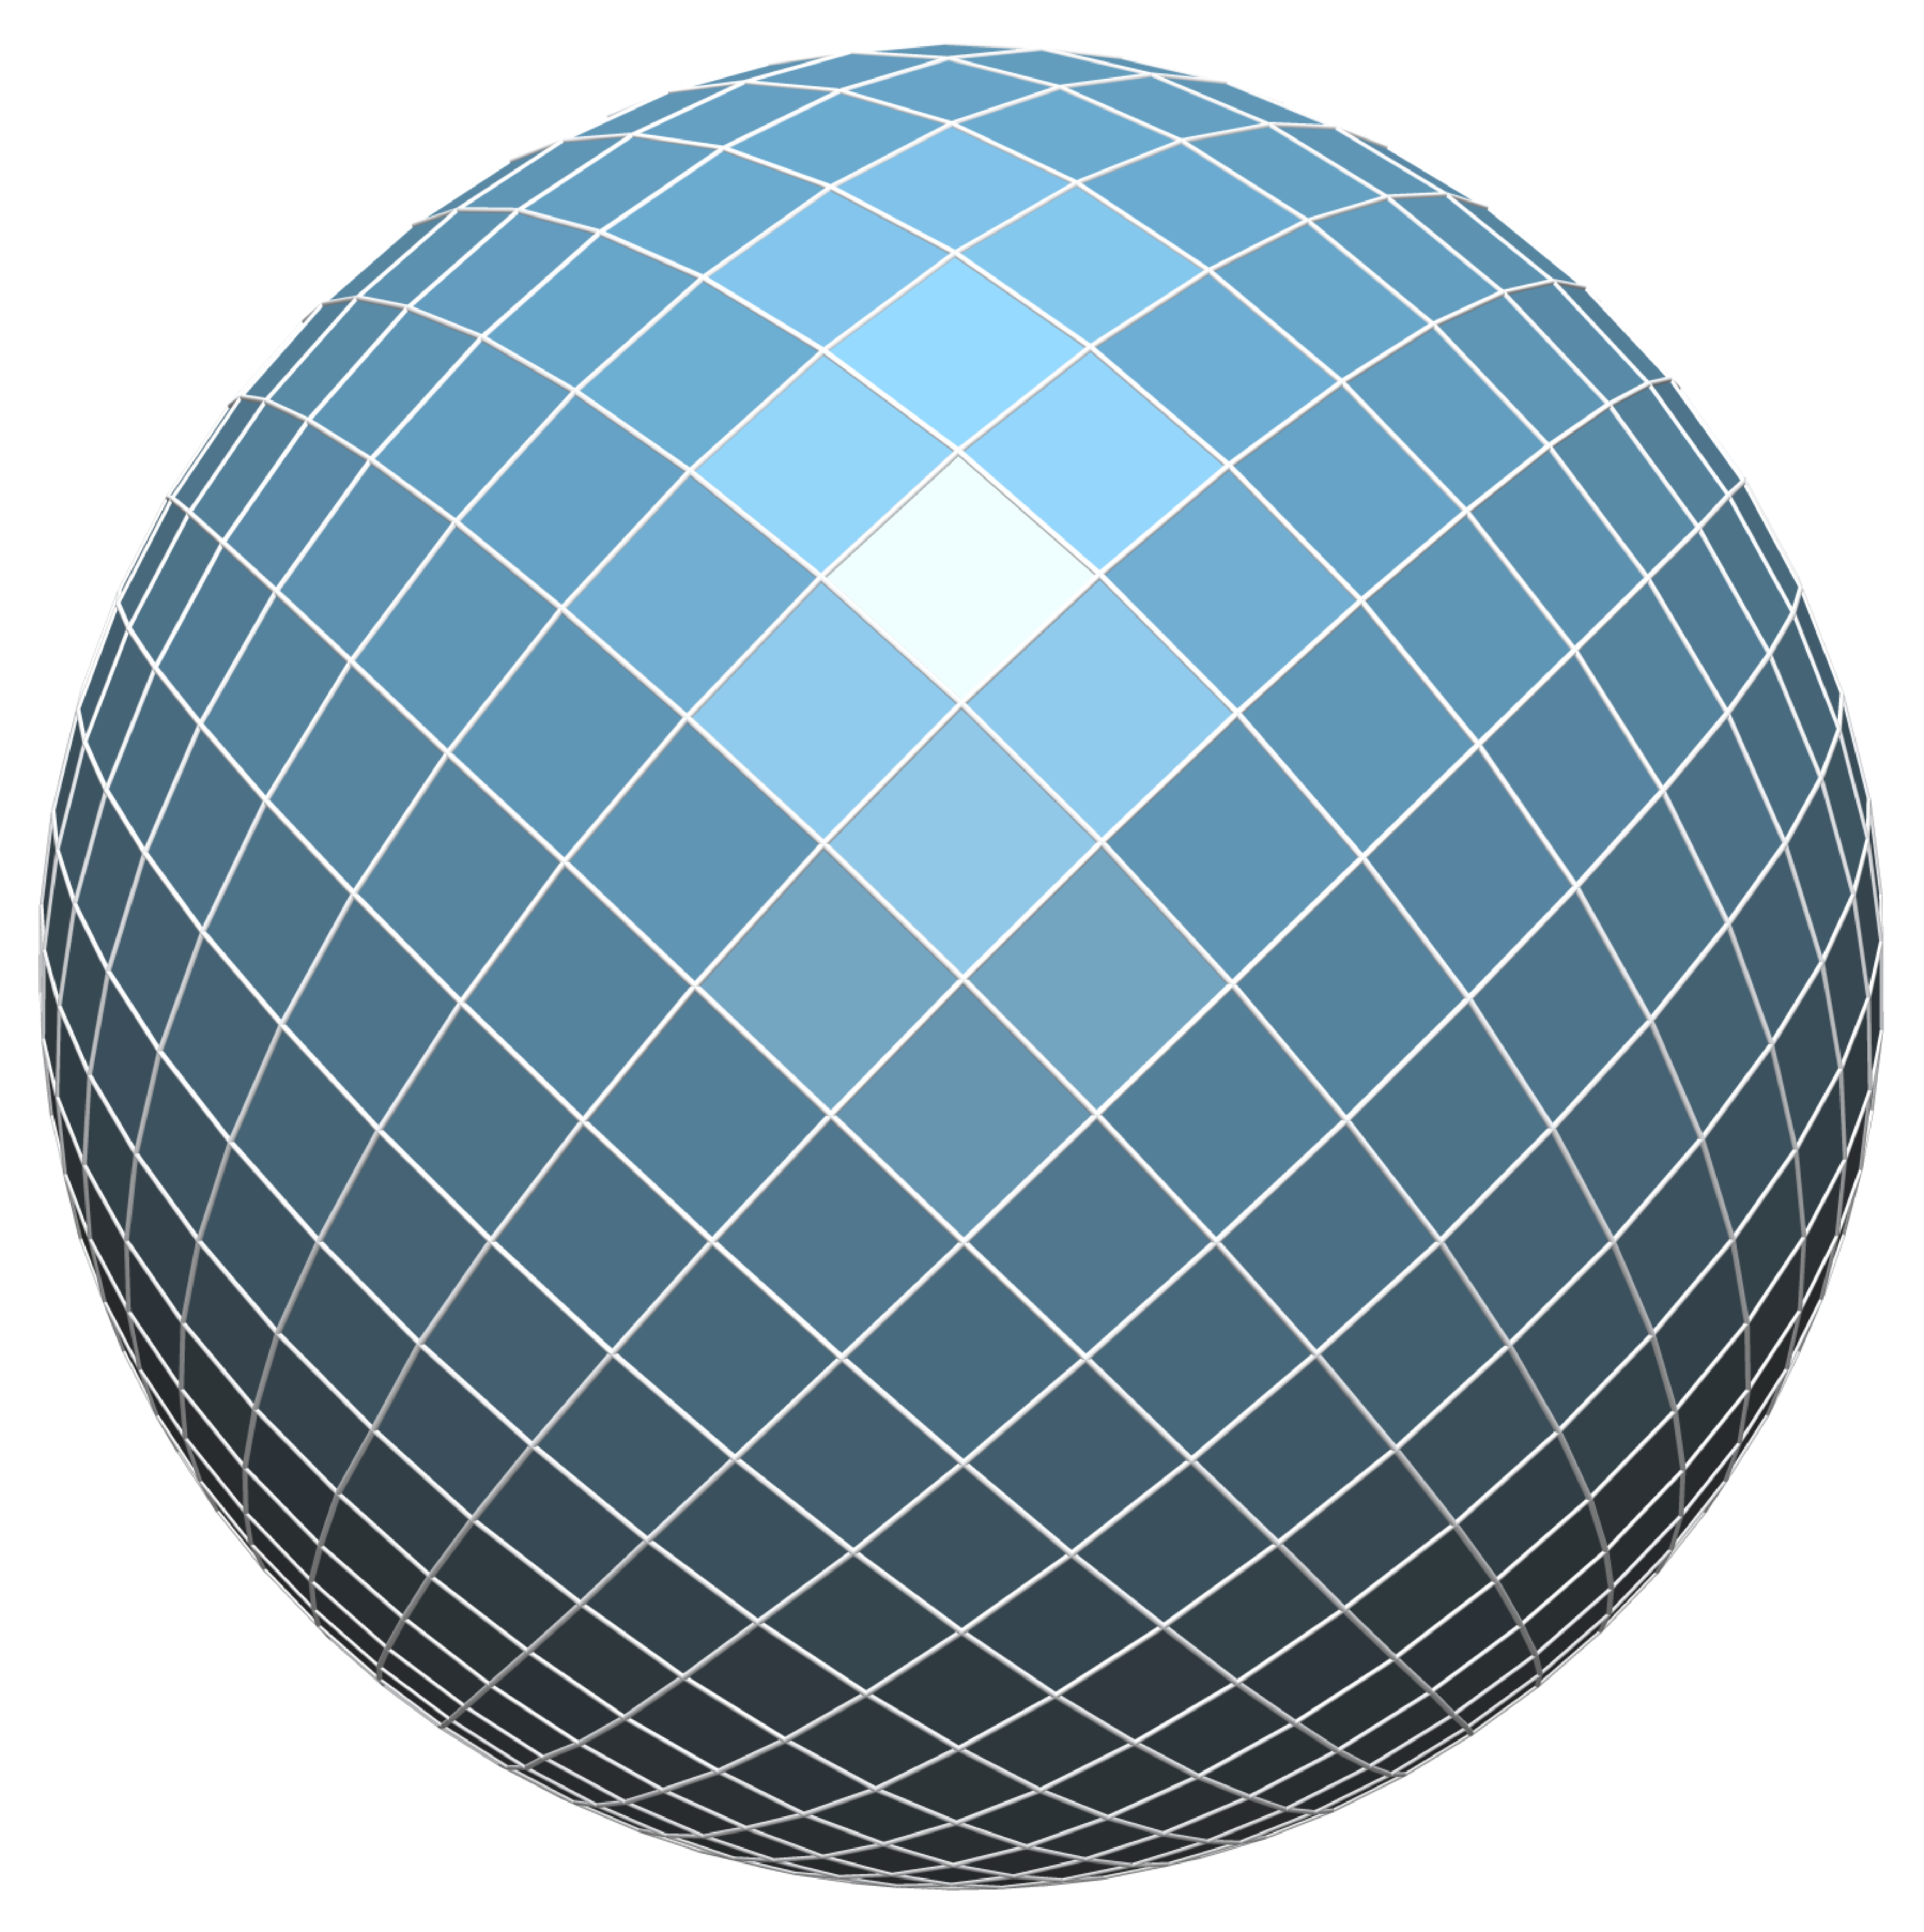
\includegraphics[width=0.32\linewidth]{images/spheres/start0_new.pdf}\\
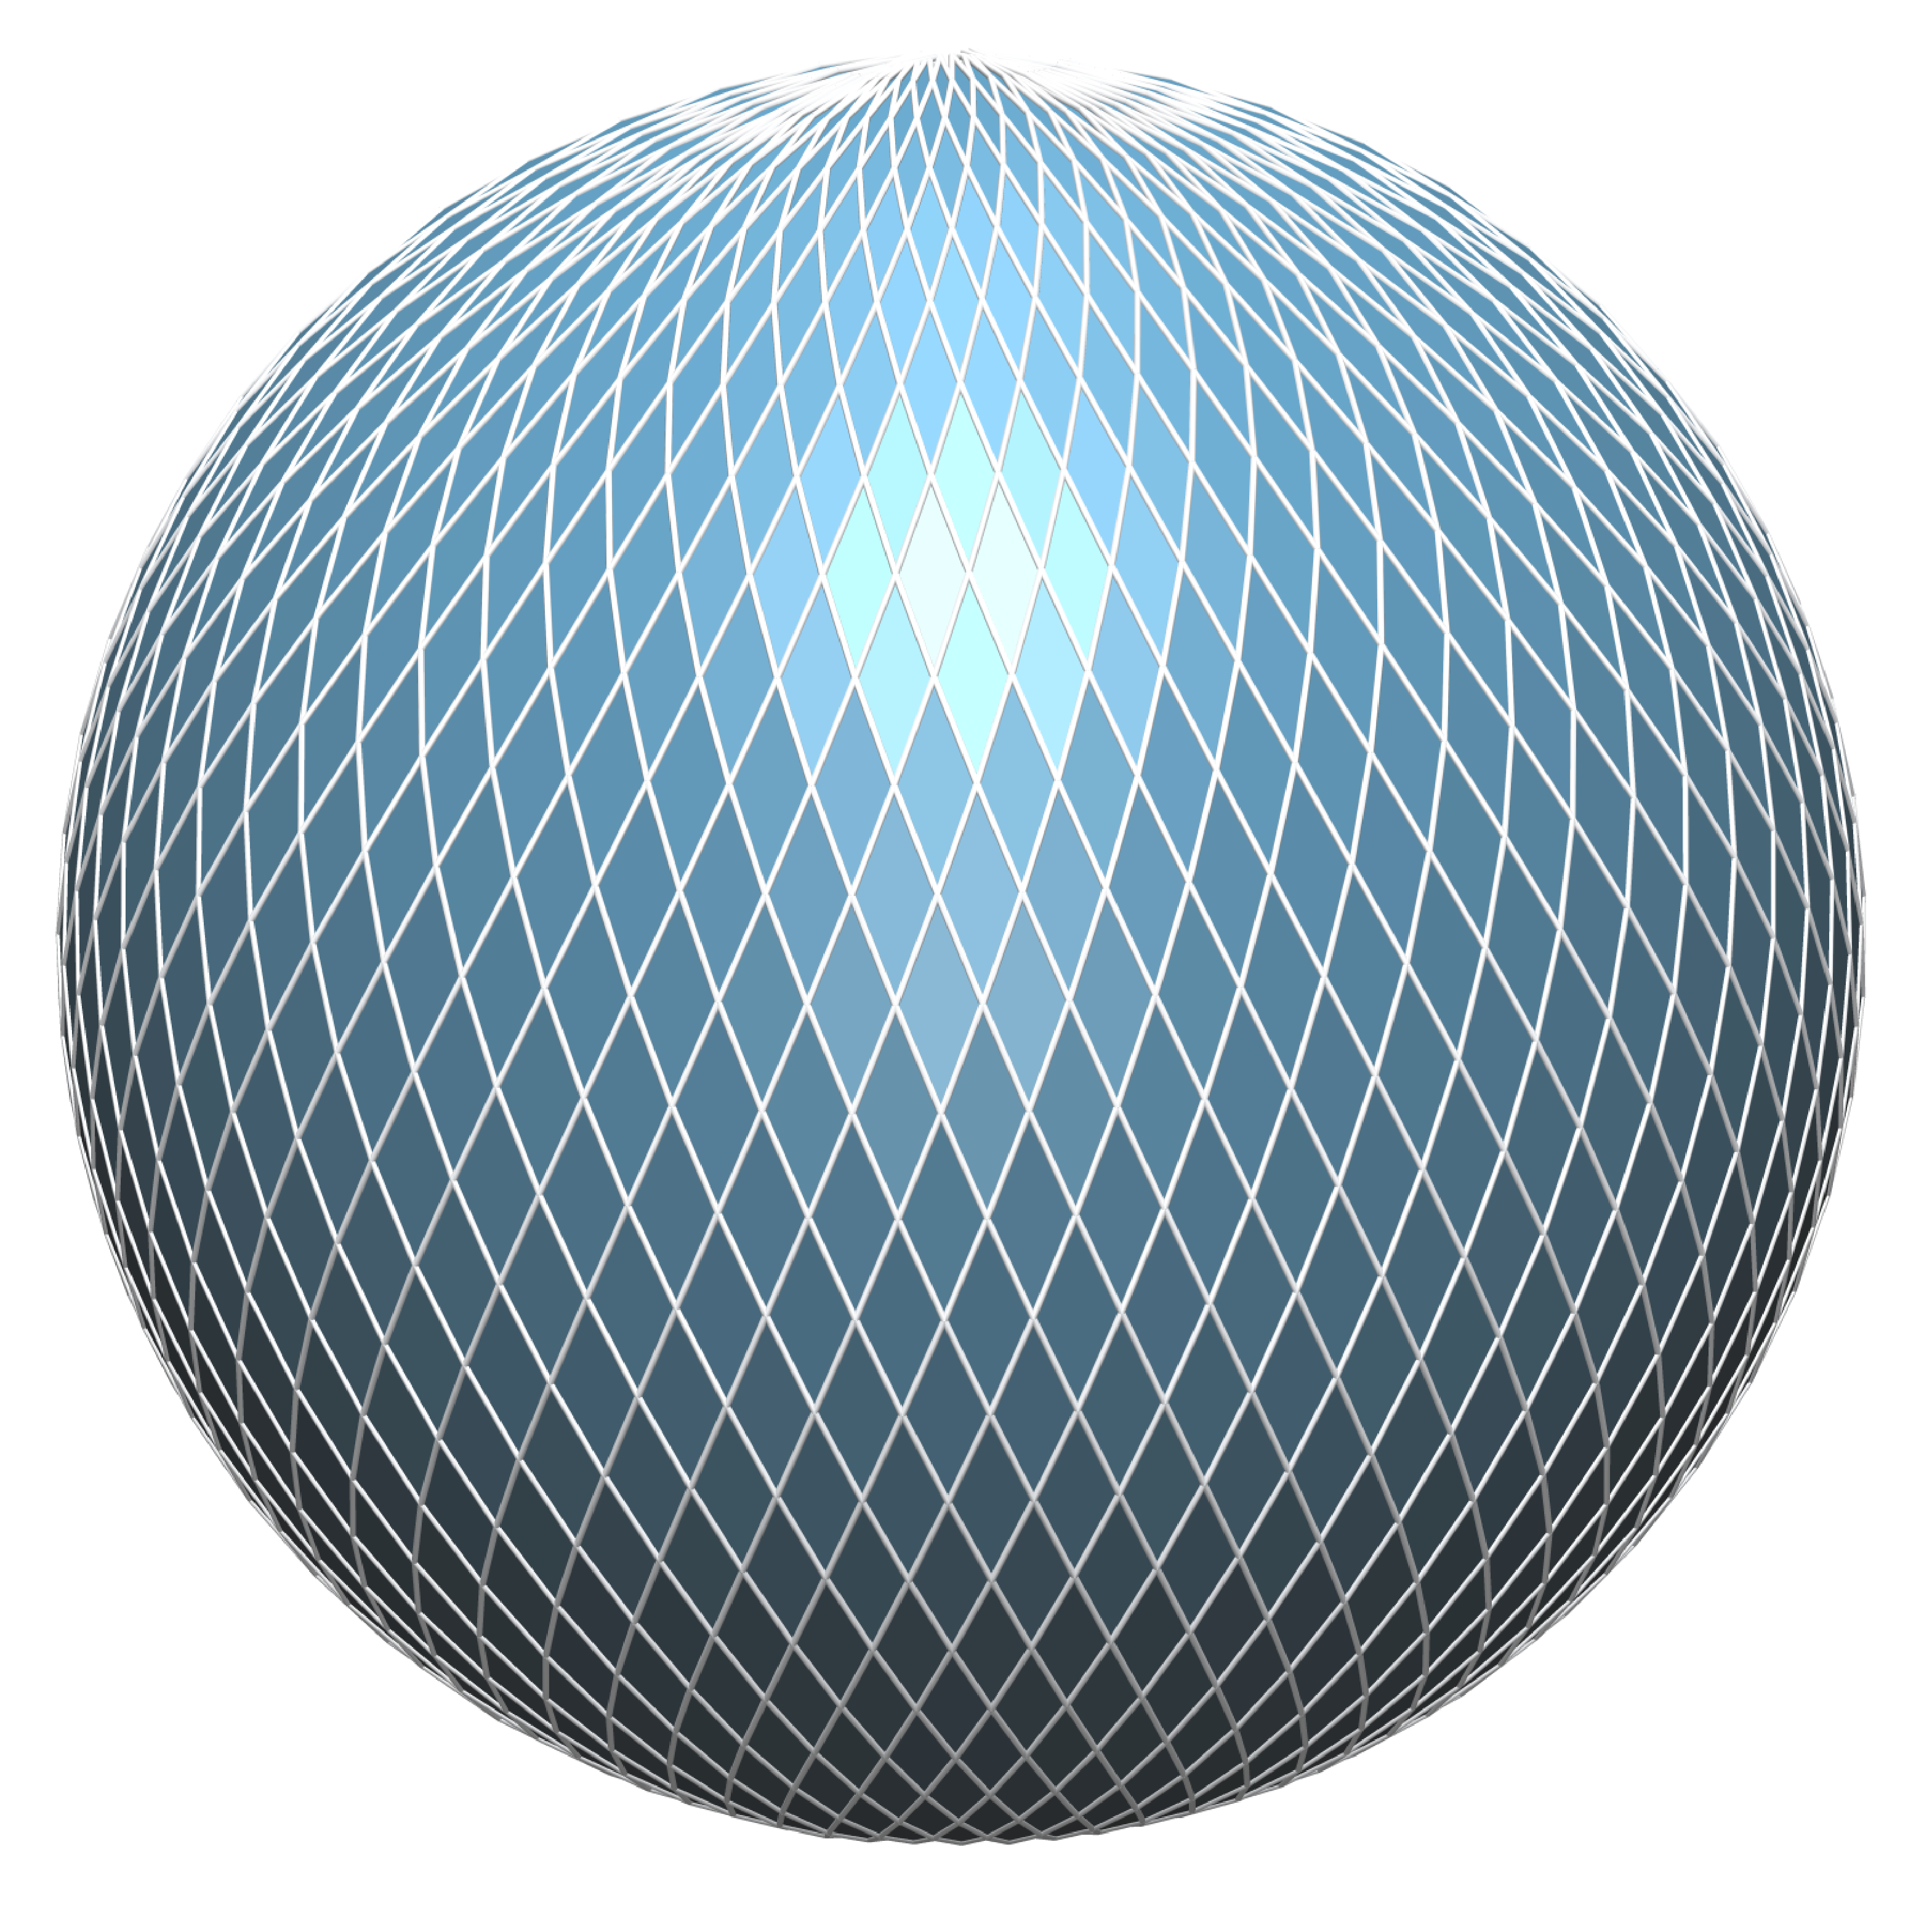
\includegraphics[width=0.32\linewidth]{images/spheres/start45_optimized_new.pdf}
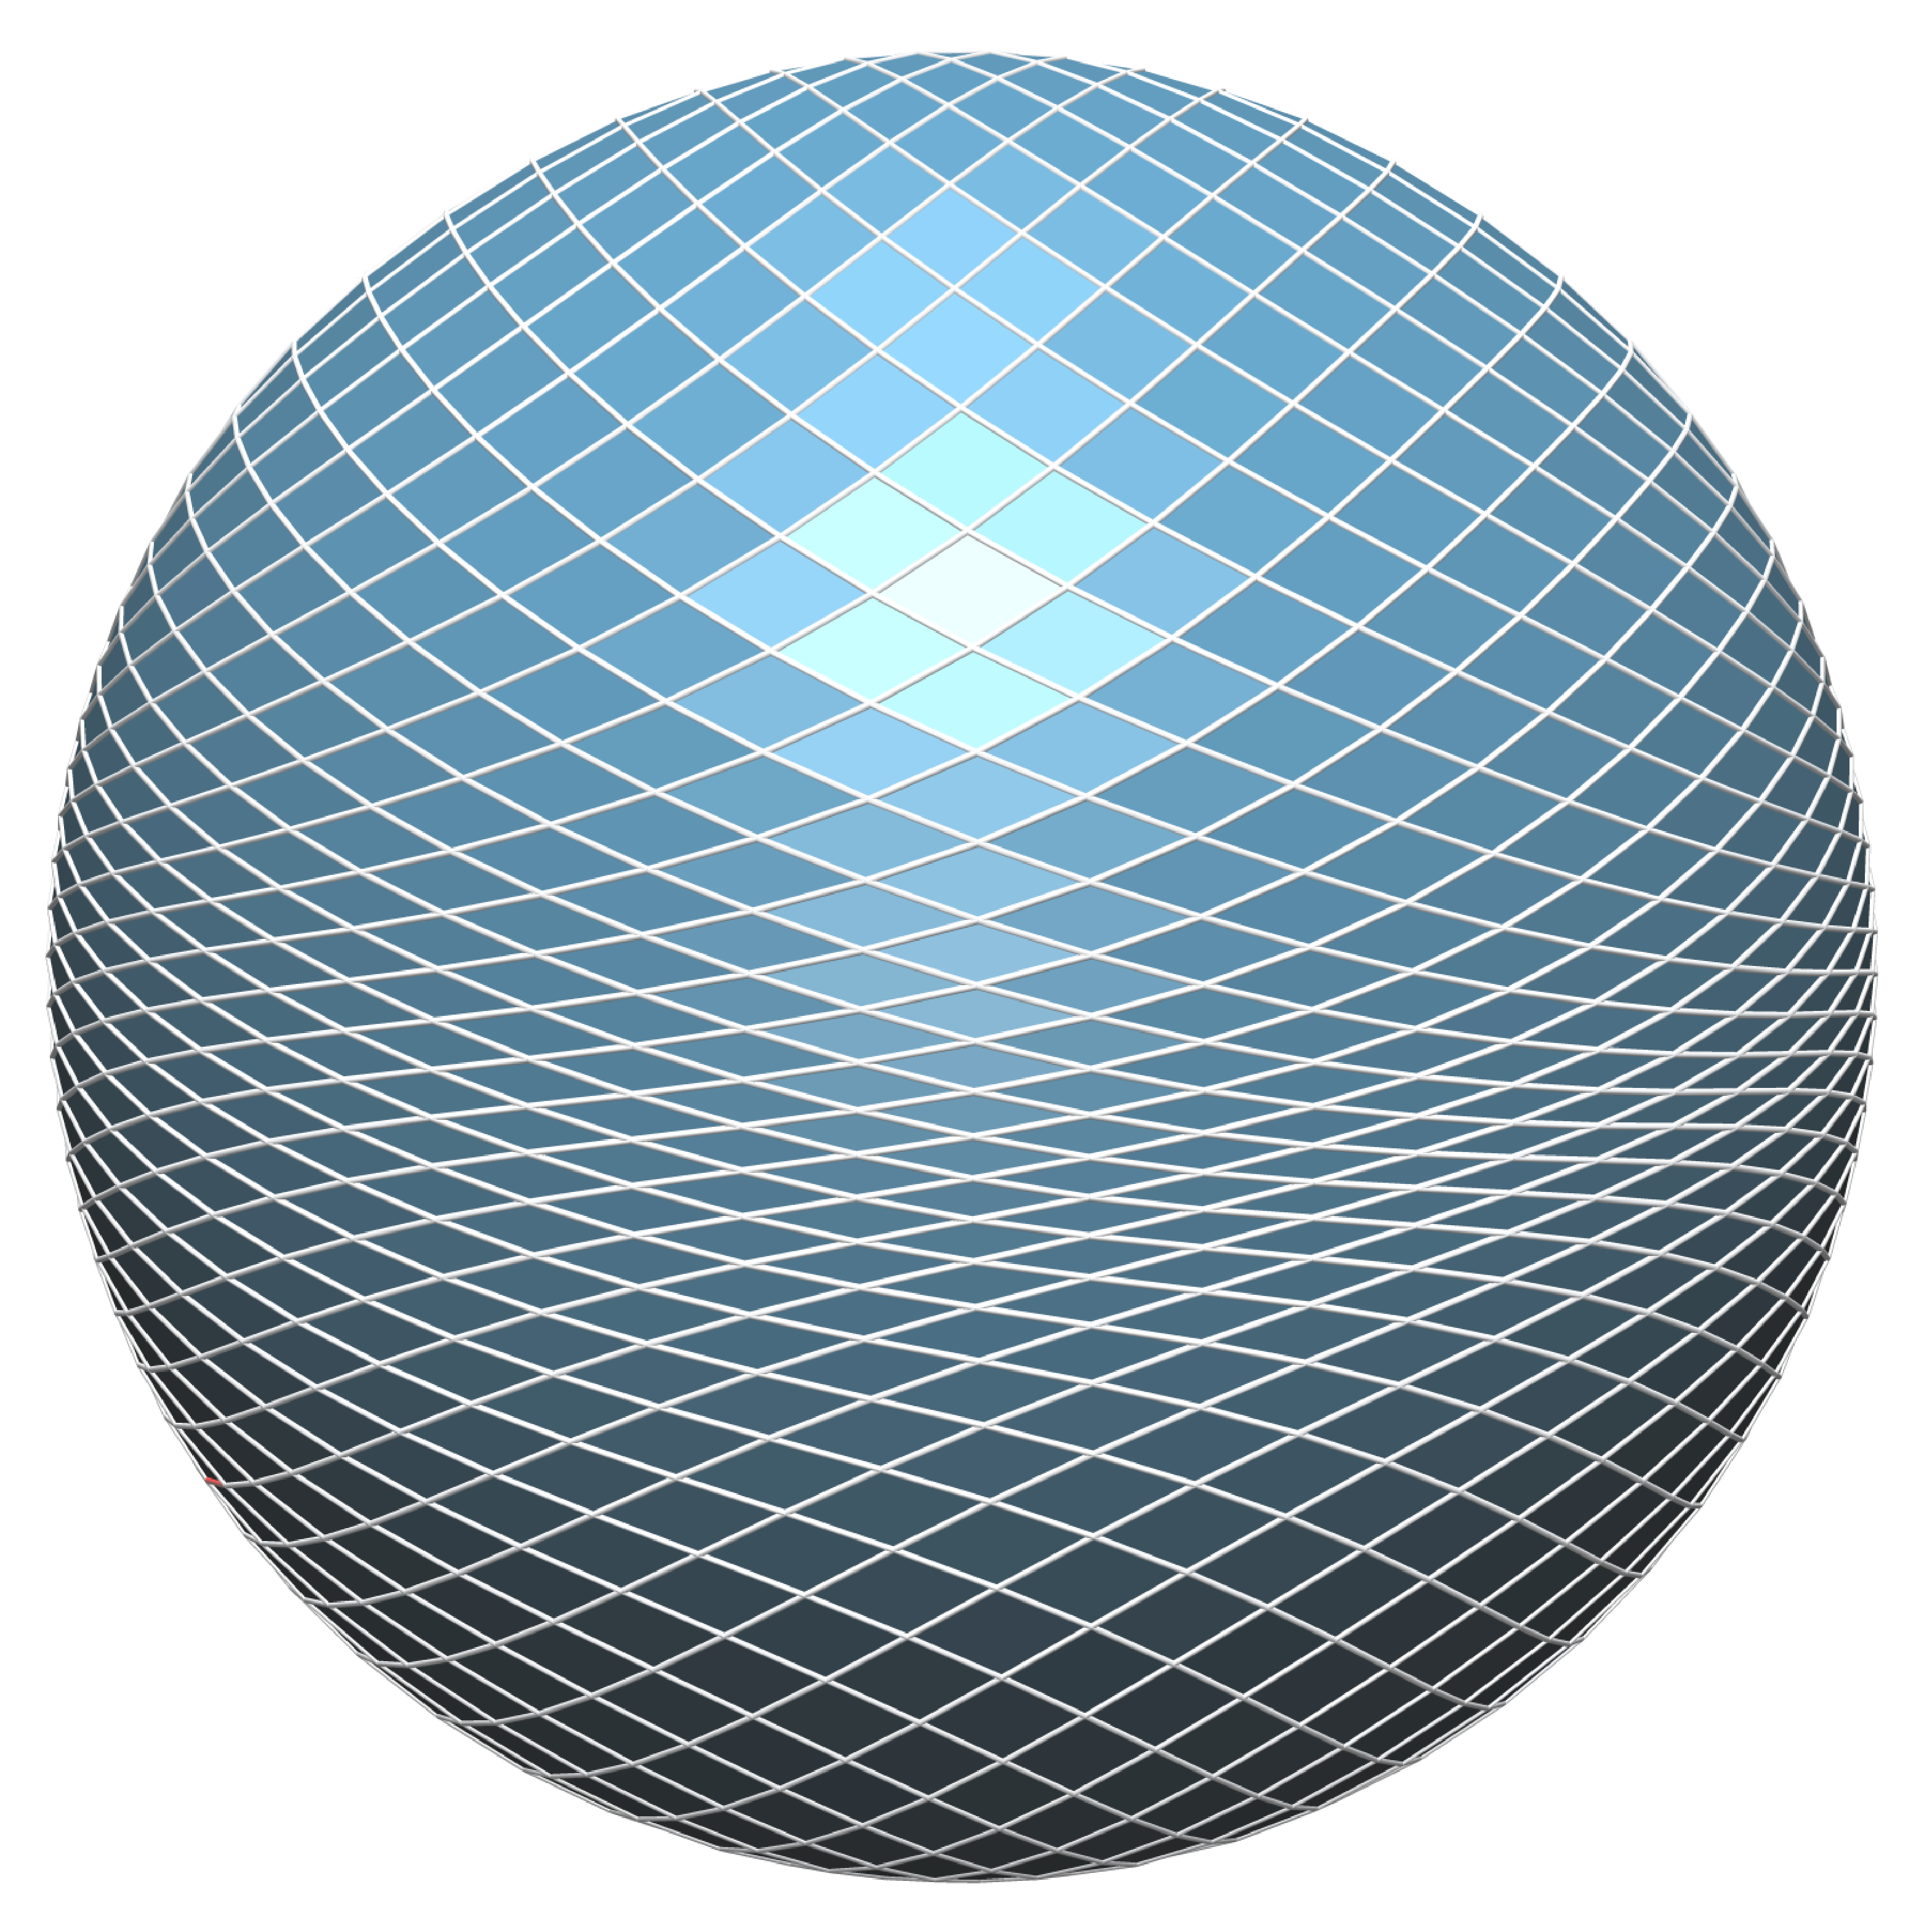
\includegraphics[width=0.32\linewidth]{images/spheres/start15_optimized_new.pdf}
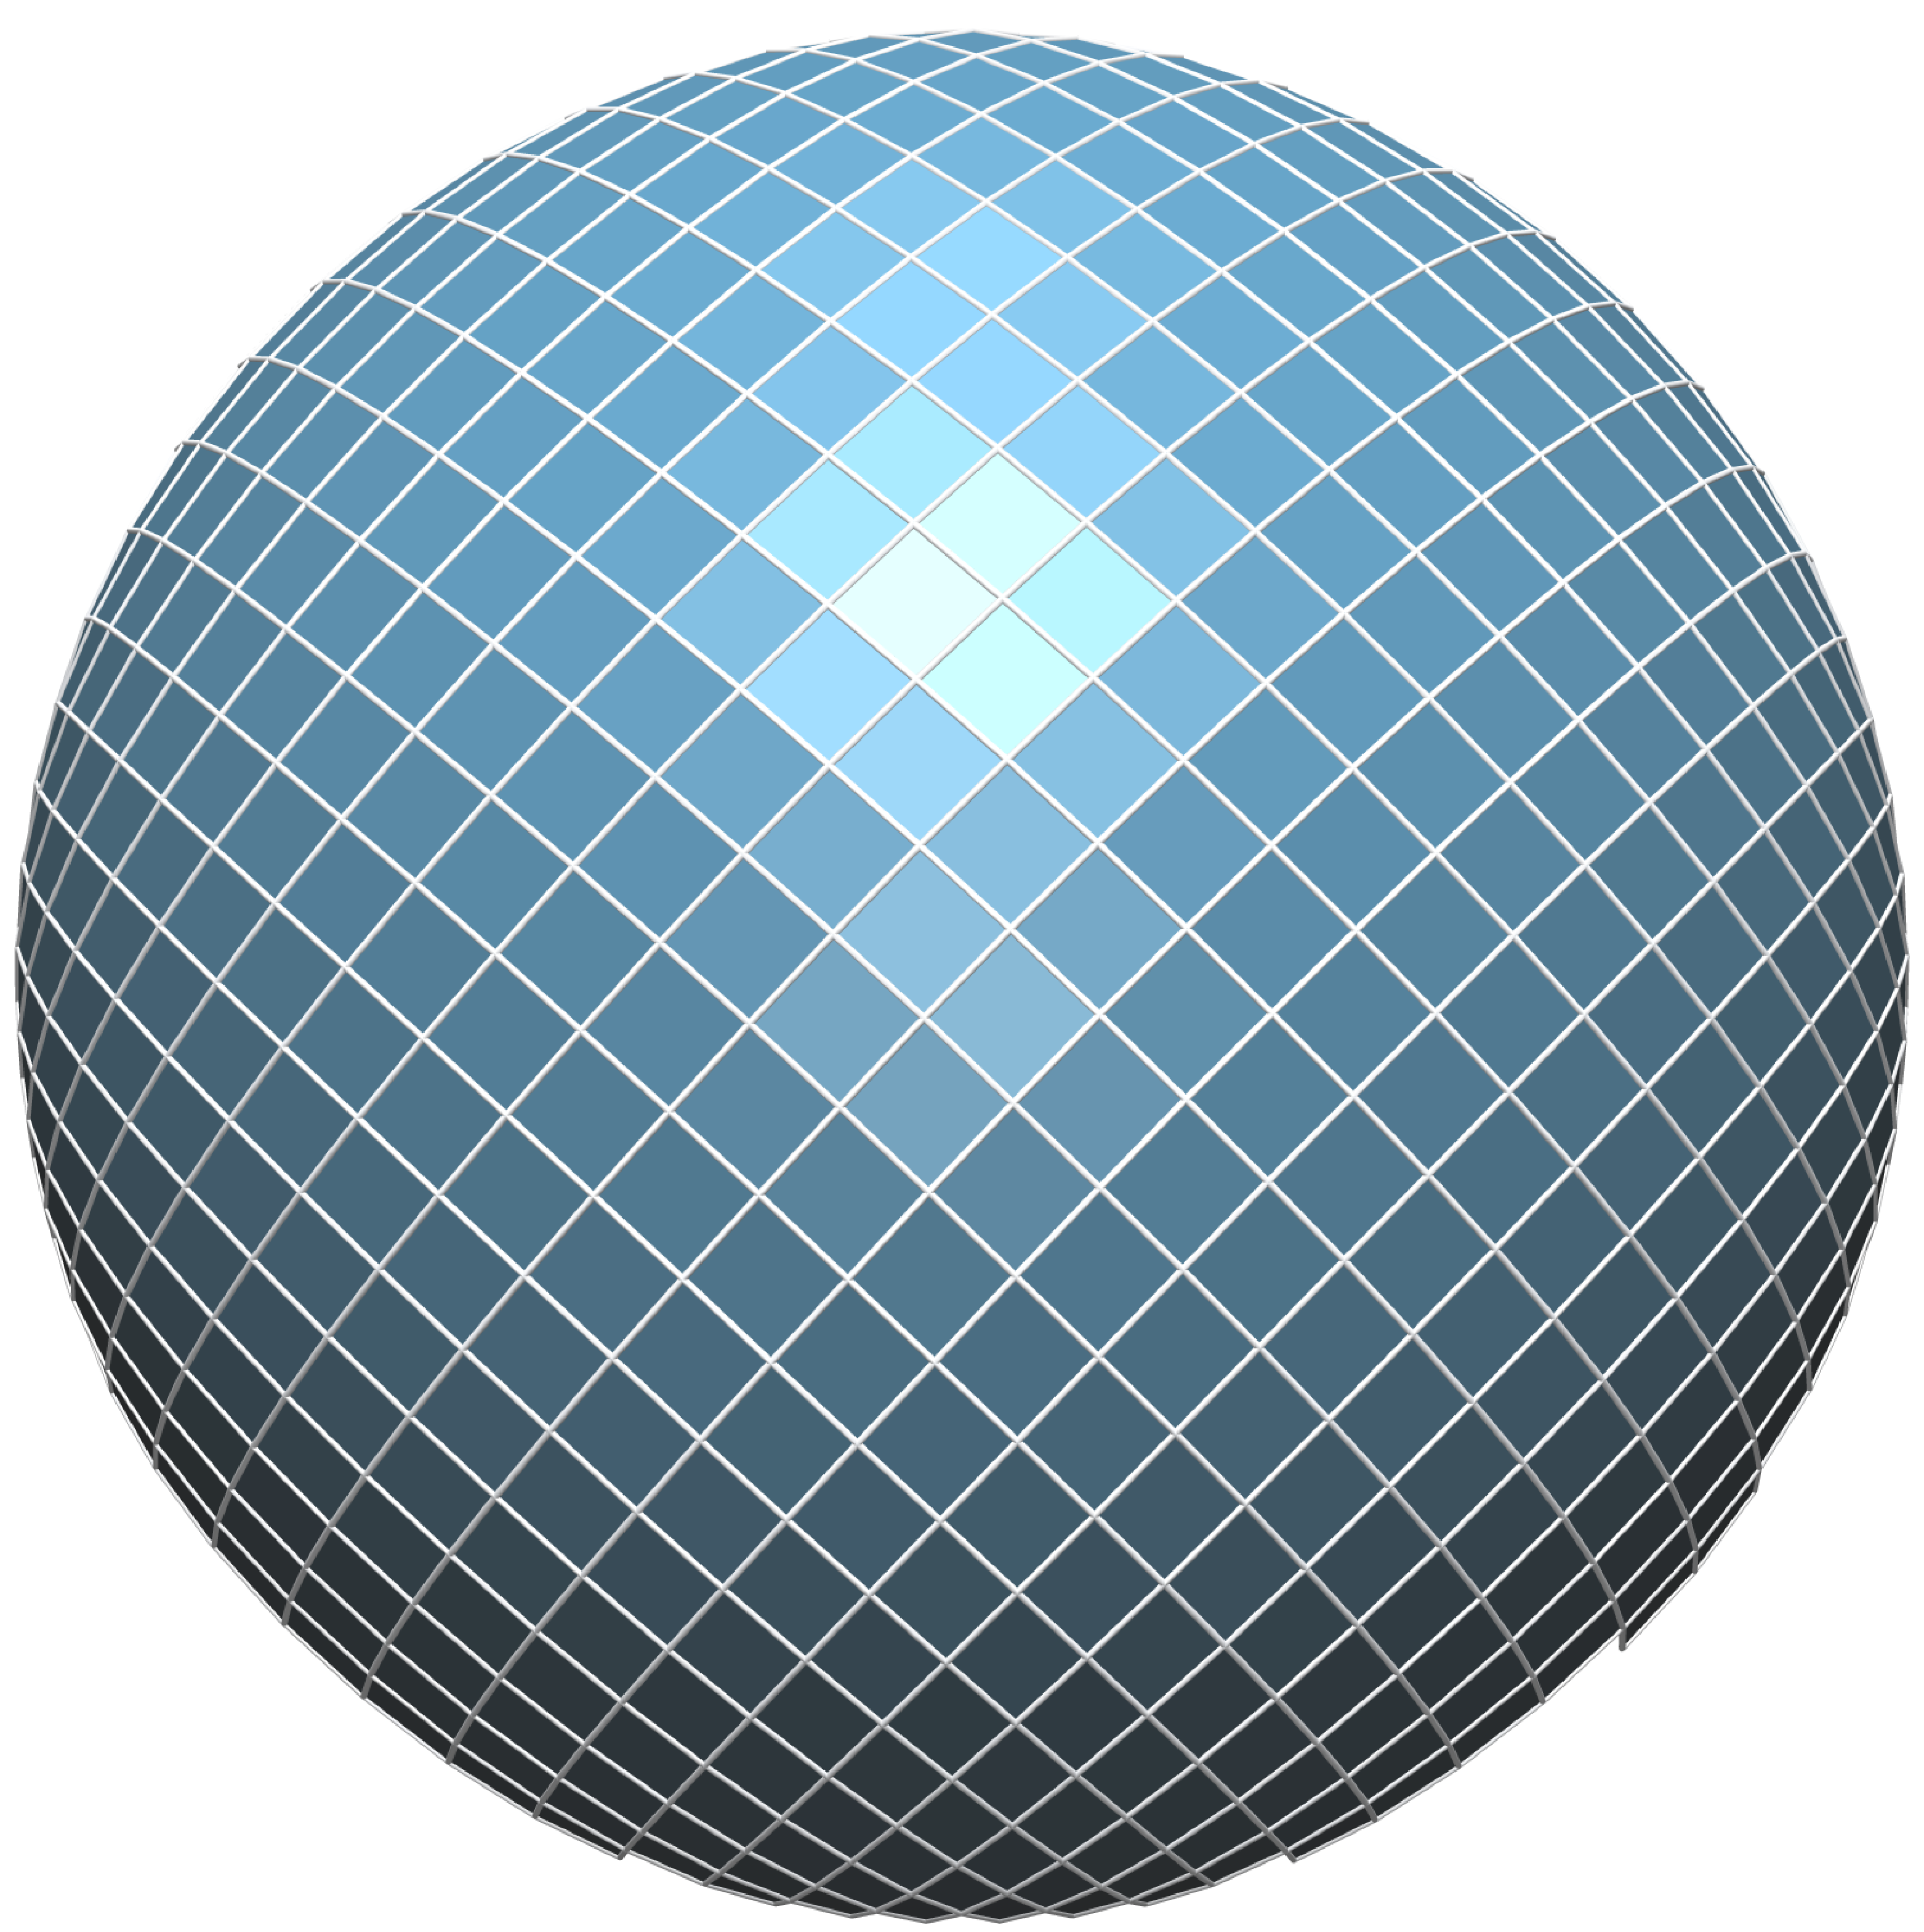
\includegraphics[width=0.32\linewidth]{images/spheres/start0_optimized_new.pdf}
\caption{Initialization meshes (top) and optimized geometries (bottom). The obtained geometry depends on the initial shear angle and on the boundary shape of the mesh. This leads to geometries that correspond visually to $k\approx 0.4$ (Fig.~\ref{fig:spheres} left), $k\approx 0.9$ (Fig.~\ref{fig:spheres} middle). For an orthogonal init mesh we obtain a solution that is not contained in the family of smooth parameterizations defined by Voss~\cite{Voss1881}. 
The edge lengths are constant and equal to $0.11$ in all solutions.}
\label{fig:spheres_optimized}
\end{figure}
As the sphere suggests there might be solutions with low curvature in the parameter curves that are not of use. In our case two angles of the quadrilaterals tend to zero with decreasing curvature. At the same time the number of edges needed for the mesh is increasing. The shear angle of the start mesh gives the family of parameterizations for the sphere and one can easily obtain a good trade-off between number of edges and curvature of the parameter curves.


\subsection{Comparison with the compass method}
Three double-curved gridshells with different types of curvature (anticlastic, synclastic and a combination of both) have been analyzed with the variational method and the results compared with the grid definitions obtained with the classic compass method. The anticlastic gridshell is between 5 and 7.5m high, 14 and 15m wide and 30m long. The synclastic gridshell is between 7.5 and 10m high, 14 and 15m wide and 30m long. Finally, the gridshell with anticlastic and synclastic curvatures, analogue to the Downland Museum gridshell in Sussex, Great Britain (2002), has a height between 7.35 and 9.50m, a width between 12.5 and 16m and a length of 50m. 

The mesh size of all three grids is 1m and the starting angle between crossing directions in the centre of the gridshells is $90^\circ$. In the compass method, the starting angle corresponds to the angle between the initial curved axes \cite{IL1974}, and in the variational method to the angle between crossing segments. A high weighting factor of the $E_{\textrm{\scriptsize{ref}}}$ energy has been chosen so that a distance from the reference surface lower than 1/500 of the span length can be maintained.

In the following pictures the grid topologies resulting from both methods are shown and compared for the three gridshell structures. The curvatures of the profiles have been calculated as the reciprocal of the radius of the circles defined by three consecutive grid nodes. The curvature distributions, calculated by the variational method in terms of $E_{\textrm{\scriptsize{cur}}}$, have been also illustrated through colored points. The size of the points is proportional to the curvature. The maximum and minimum curvatures correspond to the red and blue colors, respectively.

On the case of the anticlastic gridshell, see Figure~\ref{fig:Compass_Anti}, the main difference between the grid topologies is located on the corners of the lateral edges. There, the topology resulting from the variational method tends to go more transversally to the front sides. Also there, the critical curvature of the grid given by the compass method is to be found. The variational method provided a grid topology with a more homogeneous curvature distribution and a maximum curvature value reduced to 87\%.

\begin{figure}
\centering
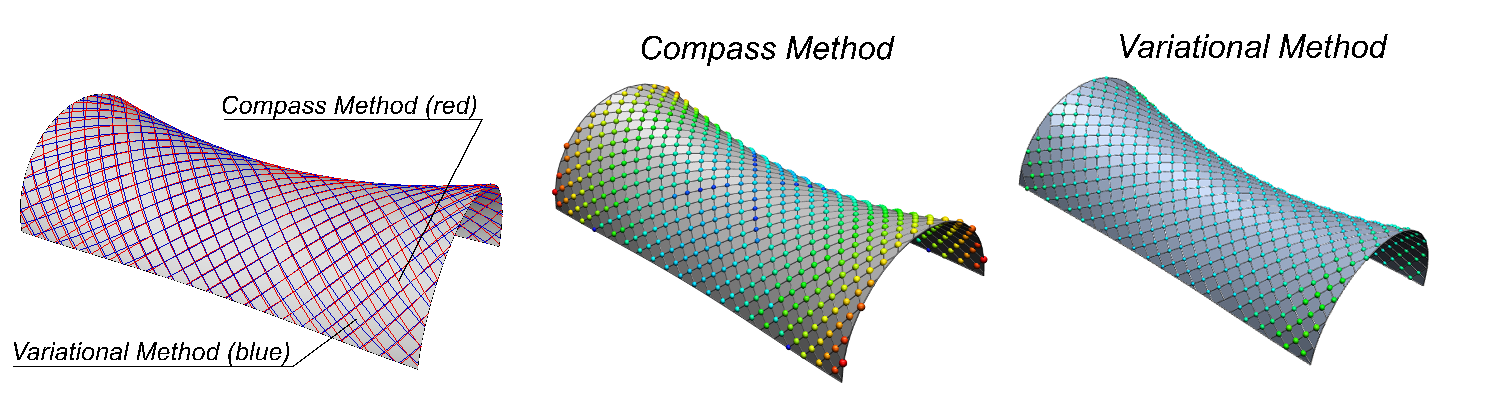
\includegraphics[width=1.0\linewidth]{images/CaseStudies_Regular/Compass_Anti.pdf}
\caption{Comparison between grid topologies for an anticlastic gridshell. The grid topology resulting from the compass method presents extreme curvature values (large red nodes) on the corners of the lateral edges. The configuration obtained with the variational method shows a more homogeneous curvature distribution and lower curvature values (smaller nodes).}
\label{fig:Compass_Anti}
\end{figure}

\begin{figure}
\centering
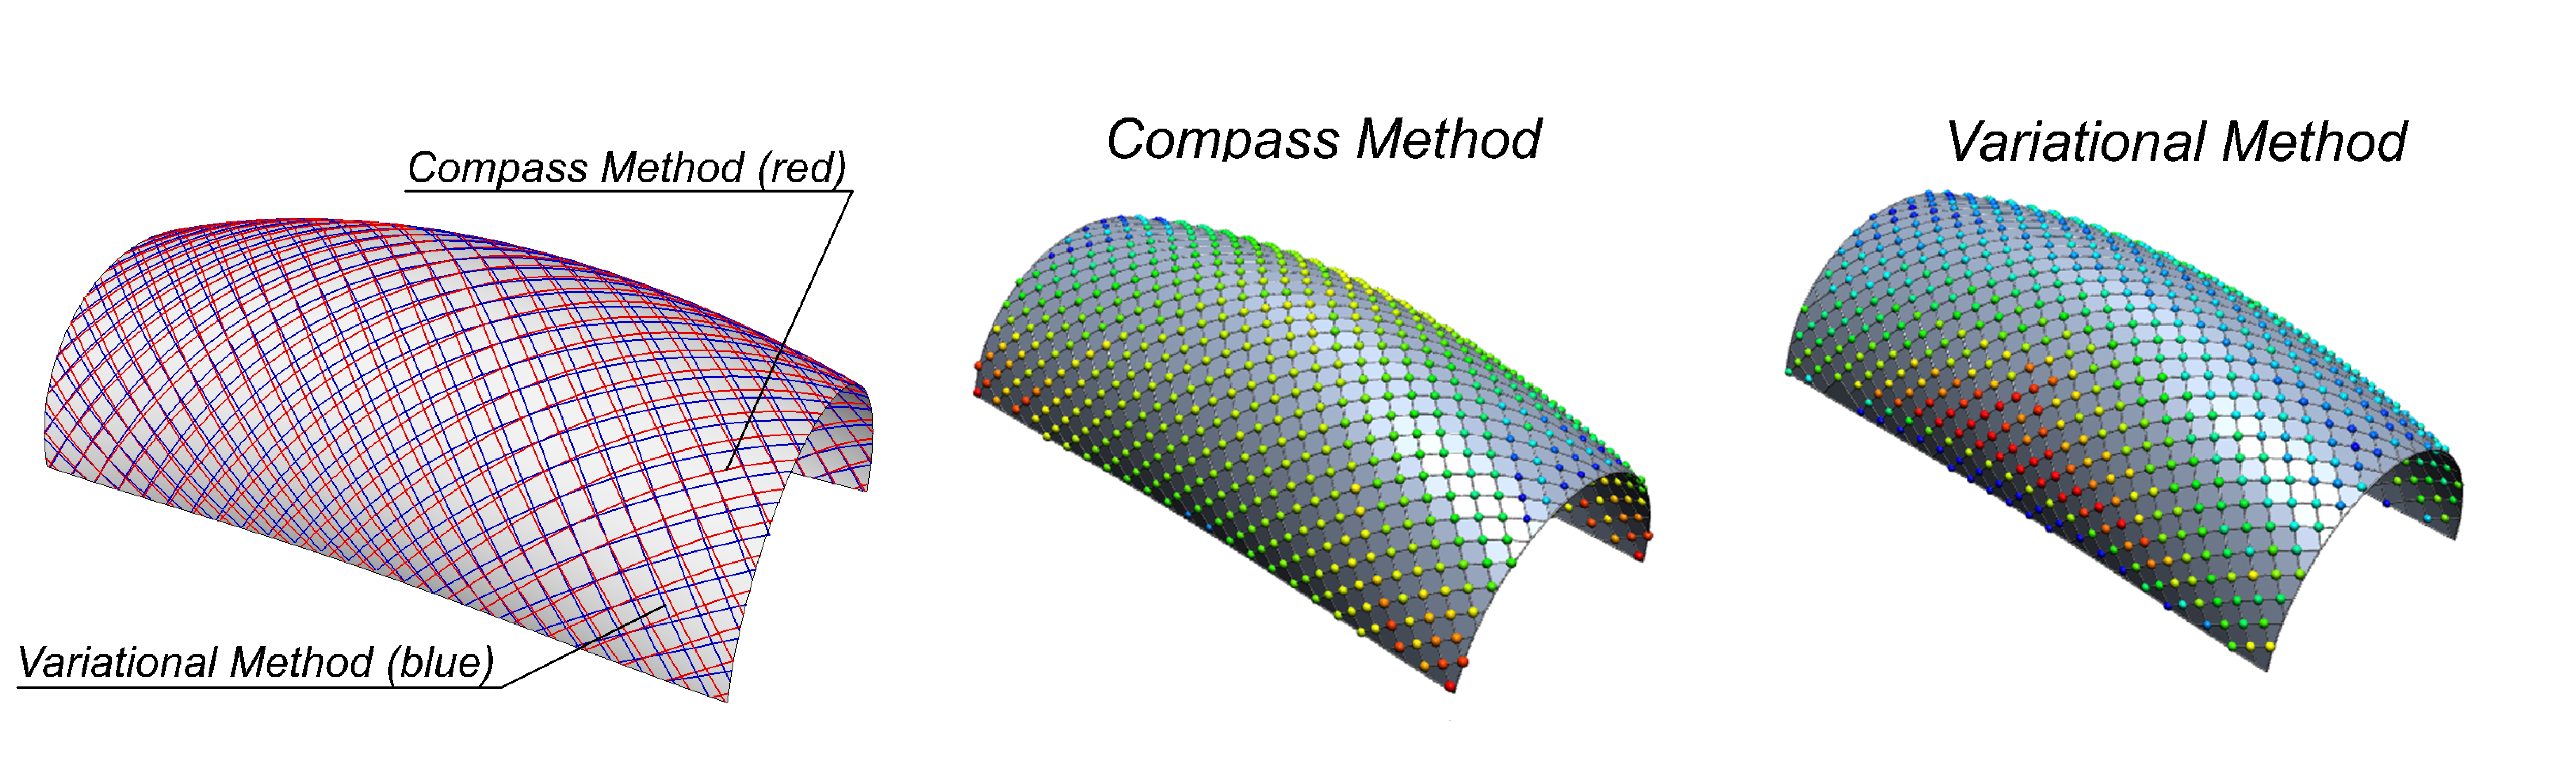
\includegraphics[width=1.0\linewidth]{images/CaseStudies_Regular/Compass_syn.pdf}
\caption{Comparison between grid topologies for a synclastic gridshell. The grid topology resulting from the compass method presents again extreme curvature values (large red nodes) on the corners of the lateral edges. The configuration obtained with the variational method owns lower maximum and mean curvature values.}
\label{fig:Compass_Syn}
\end{figure}

On the case of the synclastic gridshell, see Figure~\ref{fig:Compass_Syn}, slight differences can be found on the whole lateral sides between the grid topologies obtained with both methods. The grid configuration given by the compass method presents extreme curvature values on the corners of the lateral edges and on the gridshell crown. The variational method provided a grid configuration with lower curvature values on the top and higher on the bottom of the gridshell, the  maximum profiles curvature could be reduced to 90\% compared to the compass method.

On the case of the gridshell analogue to the Downland Museum, see Figure~\ref{fig:Compass_Downland}, differences between the grid topologies increase when approaching to the face sides. In both methods, higher curvature values are to be found on the crowns and lower on the valleys. By the grid resulting from the variational method, extreme curvature values are less concentrated as in the compass method configuration. The maximum profiles curvature could be minimized to 88\%.

\begin{figure}
\centering
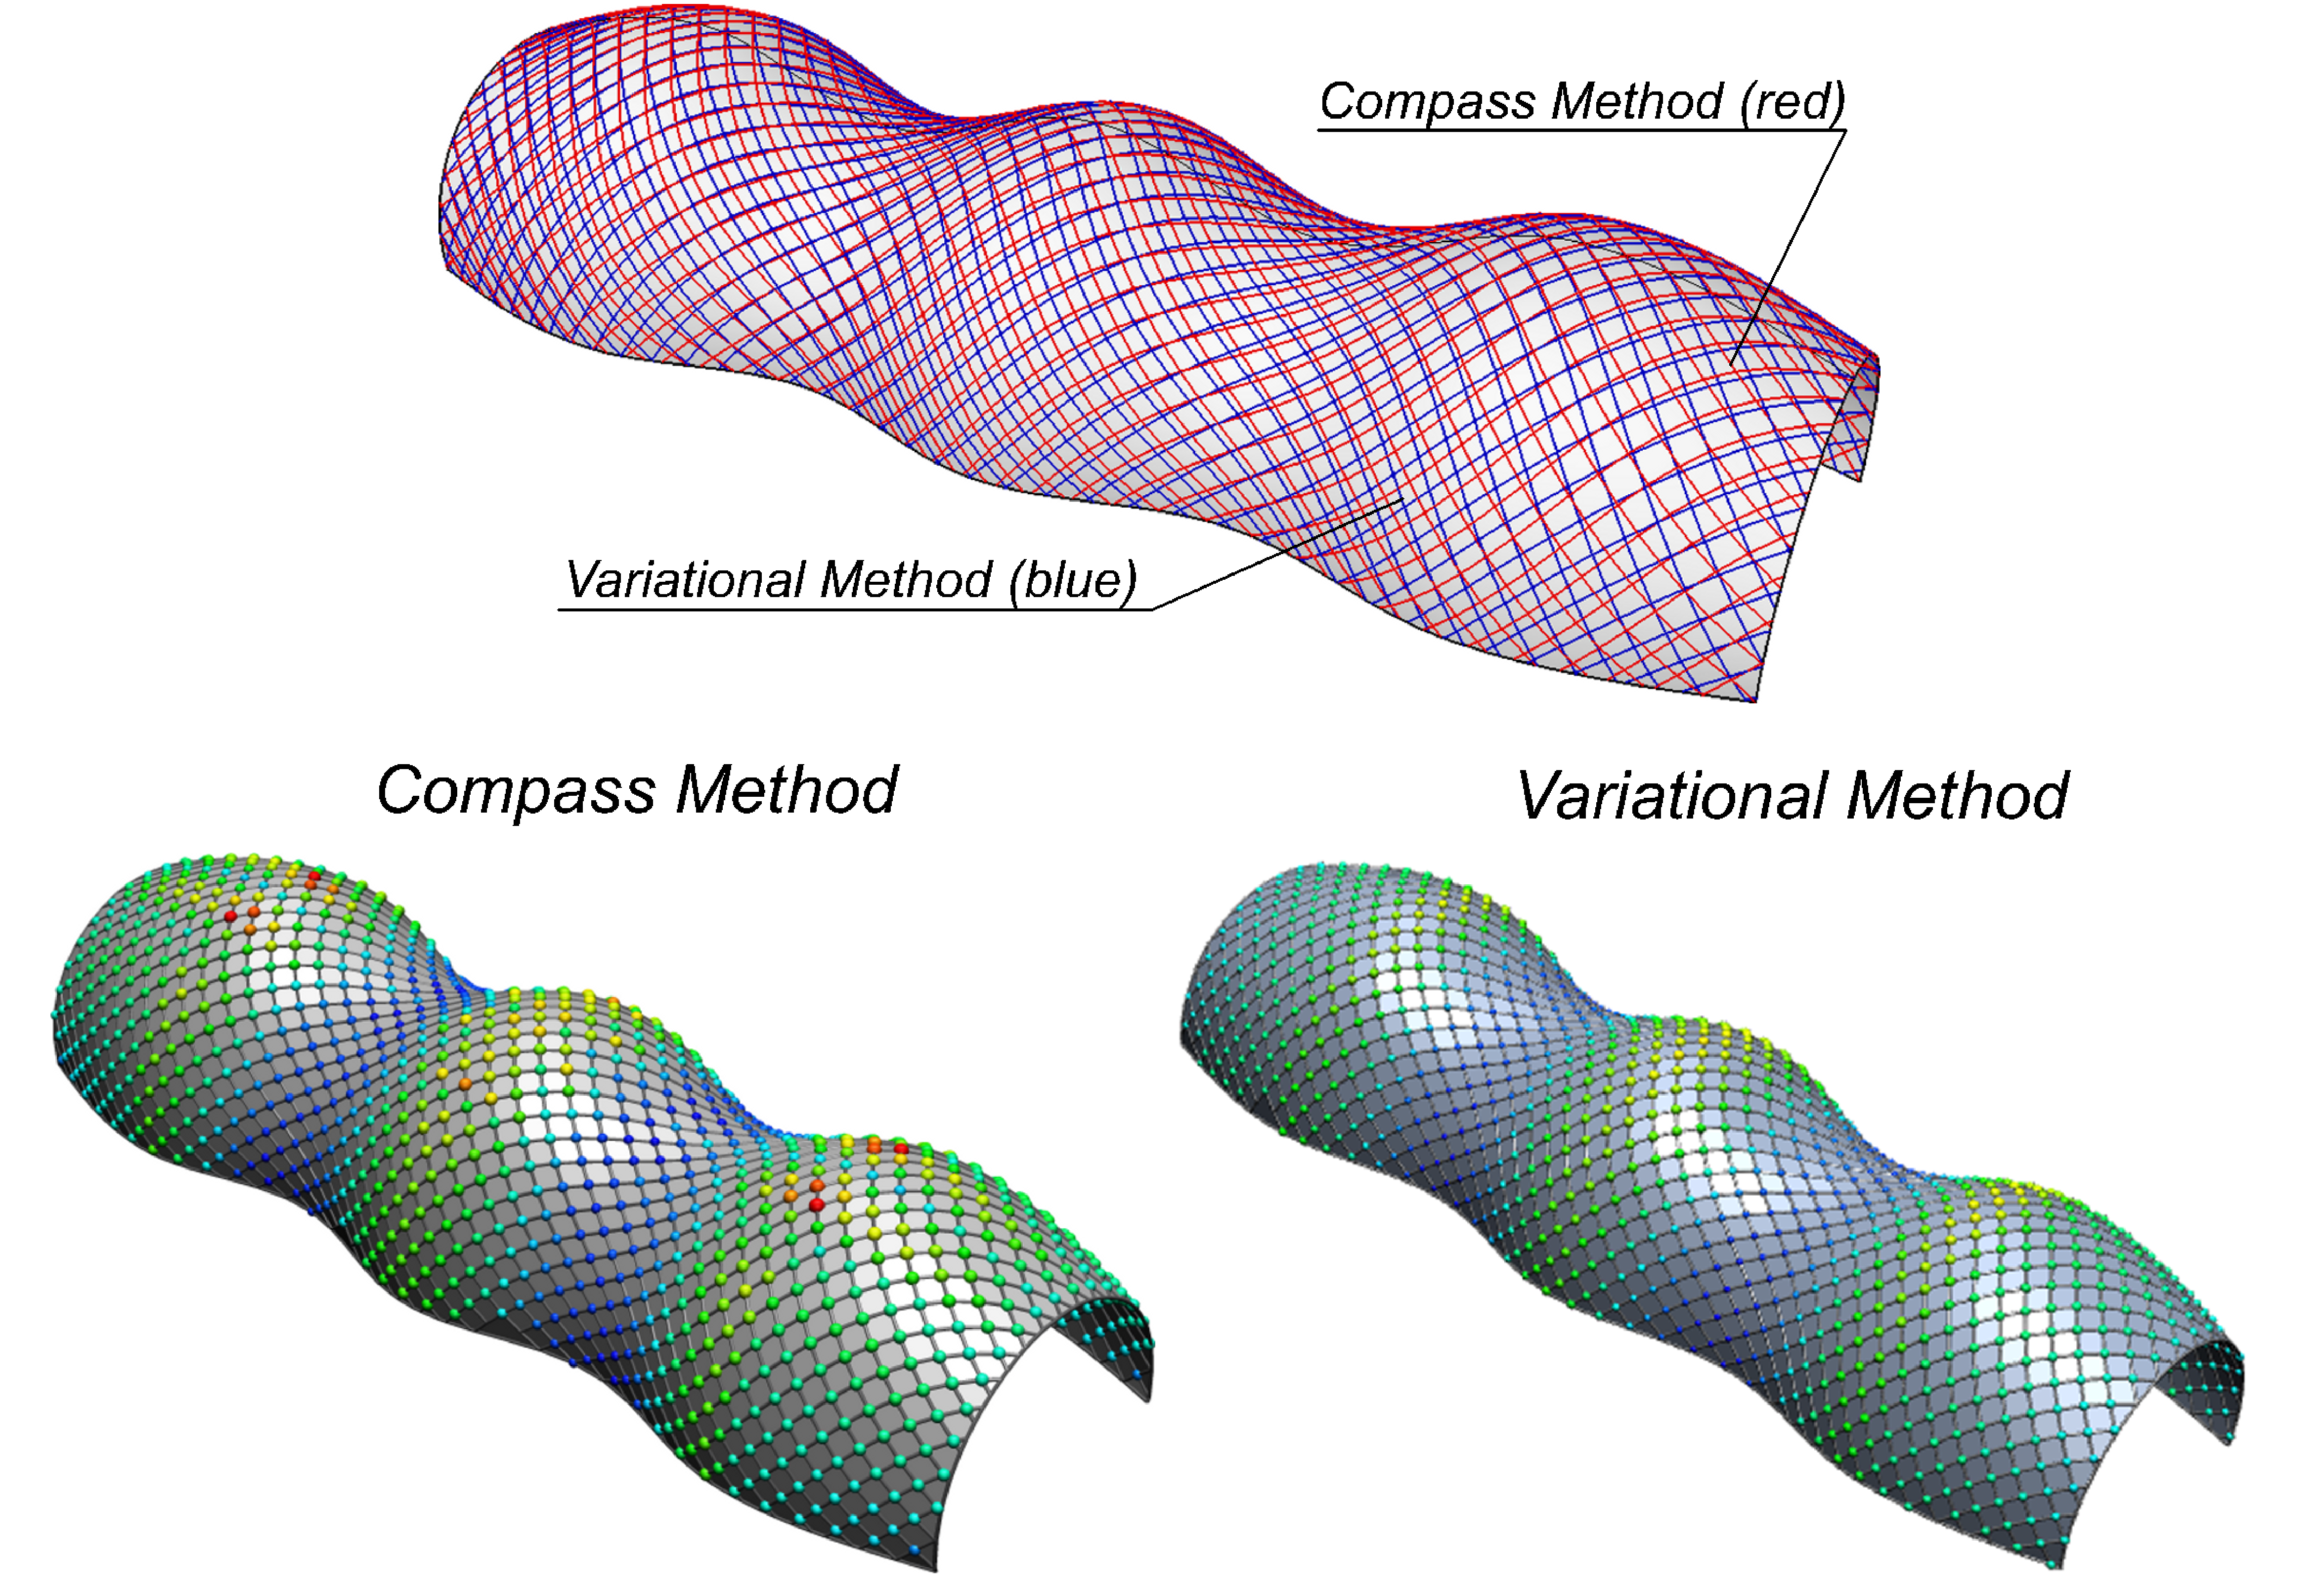
\includegraphics[width=0.80\linewidth]{images/CaseStudies_Regular/Compass_Downland.pdf}
\caption{Comparison between grid topologies for the Downland-like gridshell. In both methods, higher curvature values are located on the crowns (red nodes) and lower on the valleys (blue nodes). With the variational method, a higher distribution of the extreme profiles curvatures could be obtained.}
\label{fig:Compass_Downland}
\end{figure}

With the variational method, grid topologies with lower and more homogeneously distributed profiles curvatures than by the compass method could be obtained. A further optimization could be achieved by using another starting mesh with different edge angles, by tolerating a higher distance from the reference surface or by allowing variation on the segment lengths. In the following chapters the weighting factors of the {it\ reference surface} and {it\ segments length} energies have been minimized in order to achieve a higher reduction of the grid curvature.

\subsection{Further optimization by allowing more distance to surface reference}

\begin{figure}
\centering
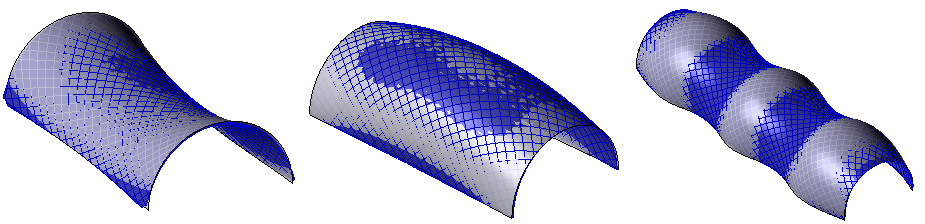
\includegraphics[width=1.0\linewidth]{images/CaseStudies_Regular/Compass_SurfaceComparison.pdf}
\caption{Deformation of the grids by allowing more distance from the reference surface}
\label{fig:Compass_SurfaceComparison}
\end{figure}

The anticlastic, synclastic and Downland-like gridshells have been further optimized by reducing the weighting factor of the {\it reference surface} energy and with it allowing a spacing between grid and target surface up to 0.6 m. Depending on the curvature distribution, the grids have been deformed above or below the reference surface.

On the case of the anticlastic gridshell, the corners of the lateral sides deform outside reducing here the maximum curvature values up to 45\% and obtaining a more homogeneous distribution on the centre of the gridshell. The mean curvature of the profiles could be reduced up to 51\%. By the synclastic gridshell, the lateral edges tend to distort outwards in the middle and the crown of the grid slightly upwards. The maximum and mean profiles curvatures were reduced up to 79\% and 78\%, respectively. By the gridshell with anticlastic and synclastic curvatures, the crowns deform inwards and the valleys outwards getting a flatter surface. The maximum and mean curvatures of the profiles could be reduced here up to 76\% and 64\%, respectively, see Figure~\ref{fig:Compass_SurfaceComparison}).

\begin{figure}
\centering
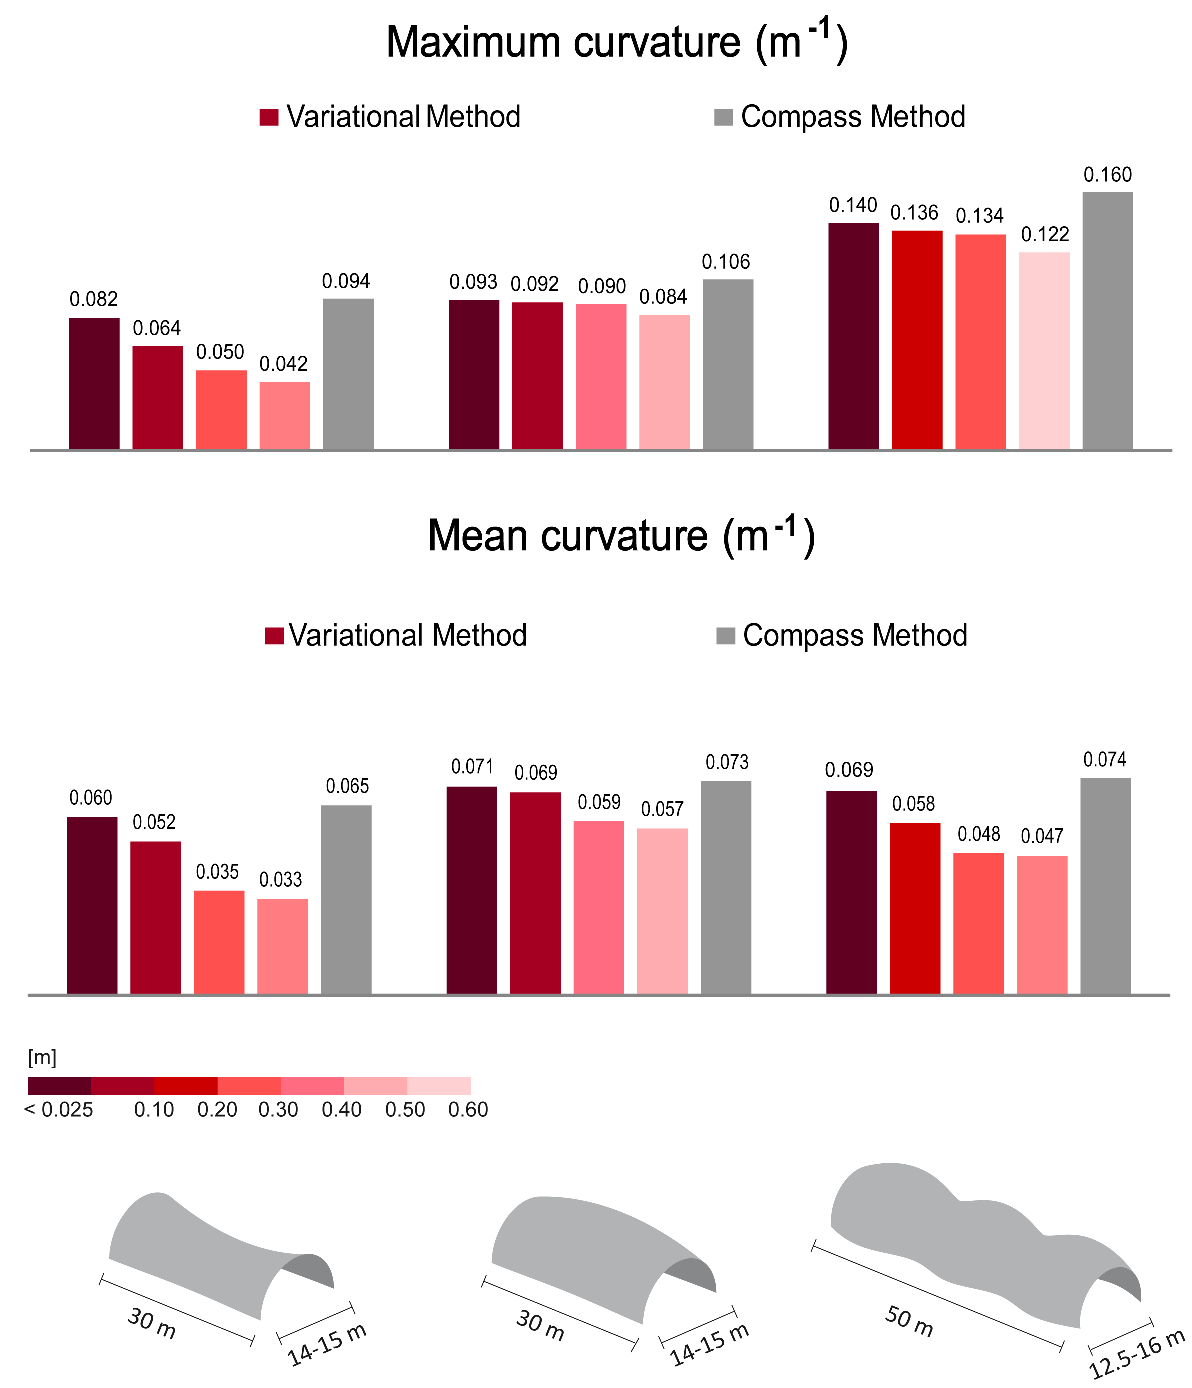
\includegraphics[width=0.80\linewidth]{images/CaseStudies_Regular/Balken.pdf}
\caption{Comparison of the maximum and mean profile curvatures of the anticlastic, synclastic and Downland-like grid topologies resulting from the variational and compass methods}
\label{fig:Balken}
\end{figure}

The diagram shown in Figure~\ref{fig:Balken} outlines the optimization results achieved with the variational method in comparison to the compass method. The maximum and mean curvatures are illustrated for the three gridshells. The color of the bars represents the distance from the reference surface. Generally, a higher reduction of the mean curvature is achieved, as the energy $E_{\textrm{\scriptsize{cur}}}$ to be minimized corresponds to the sum of all curvature values.

\section{Case studies irregular gridshells}

\subsection{Further optimization allowing variation on the segments length}

A further optimization can also be achieved by allowing the distance between grid nodes to vary, reducing thus the curvature on the grid locally and globally. A spherical calotte of 15m diameter and 10m height has been firstly optimized, with constant segment length (regular gridshell) and a starting angle between profiles of $67.5^\circ$, and afterwards  by letting the segment lengths progressively differ (irregular gridshell). 

On the case of the calotte with regular mesh, due to the characteristic polar singularities of the spheres, strong local concentrations of curvature can be observed. By letting the mesh size vary, the segment lengths become shorter on the poles and the also typical alignment in S of the grid tends to disappear, see Figure~\ref{fig:SphereIrregular}.

\begin{figure}
\centering
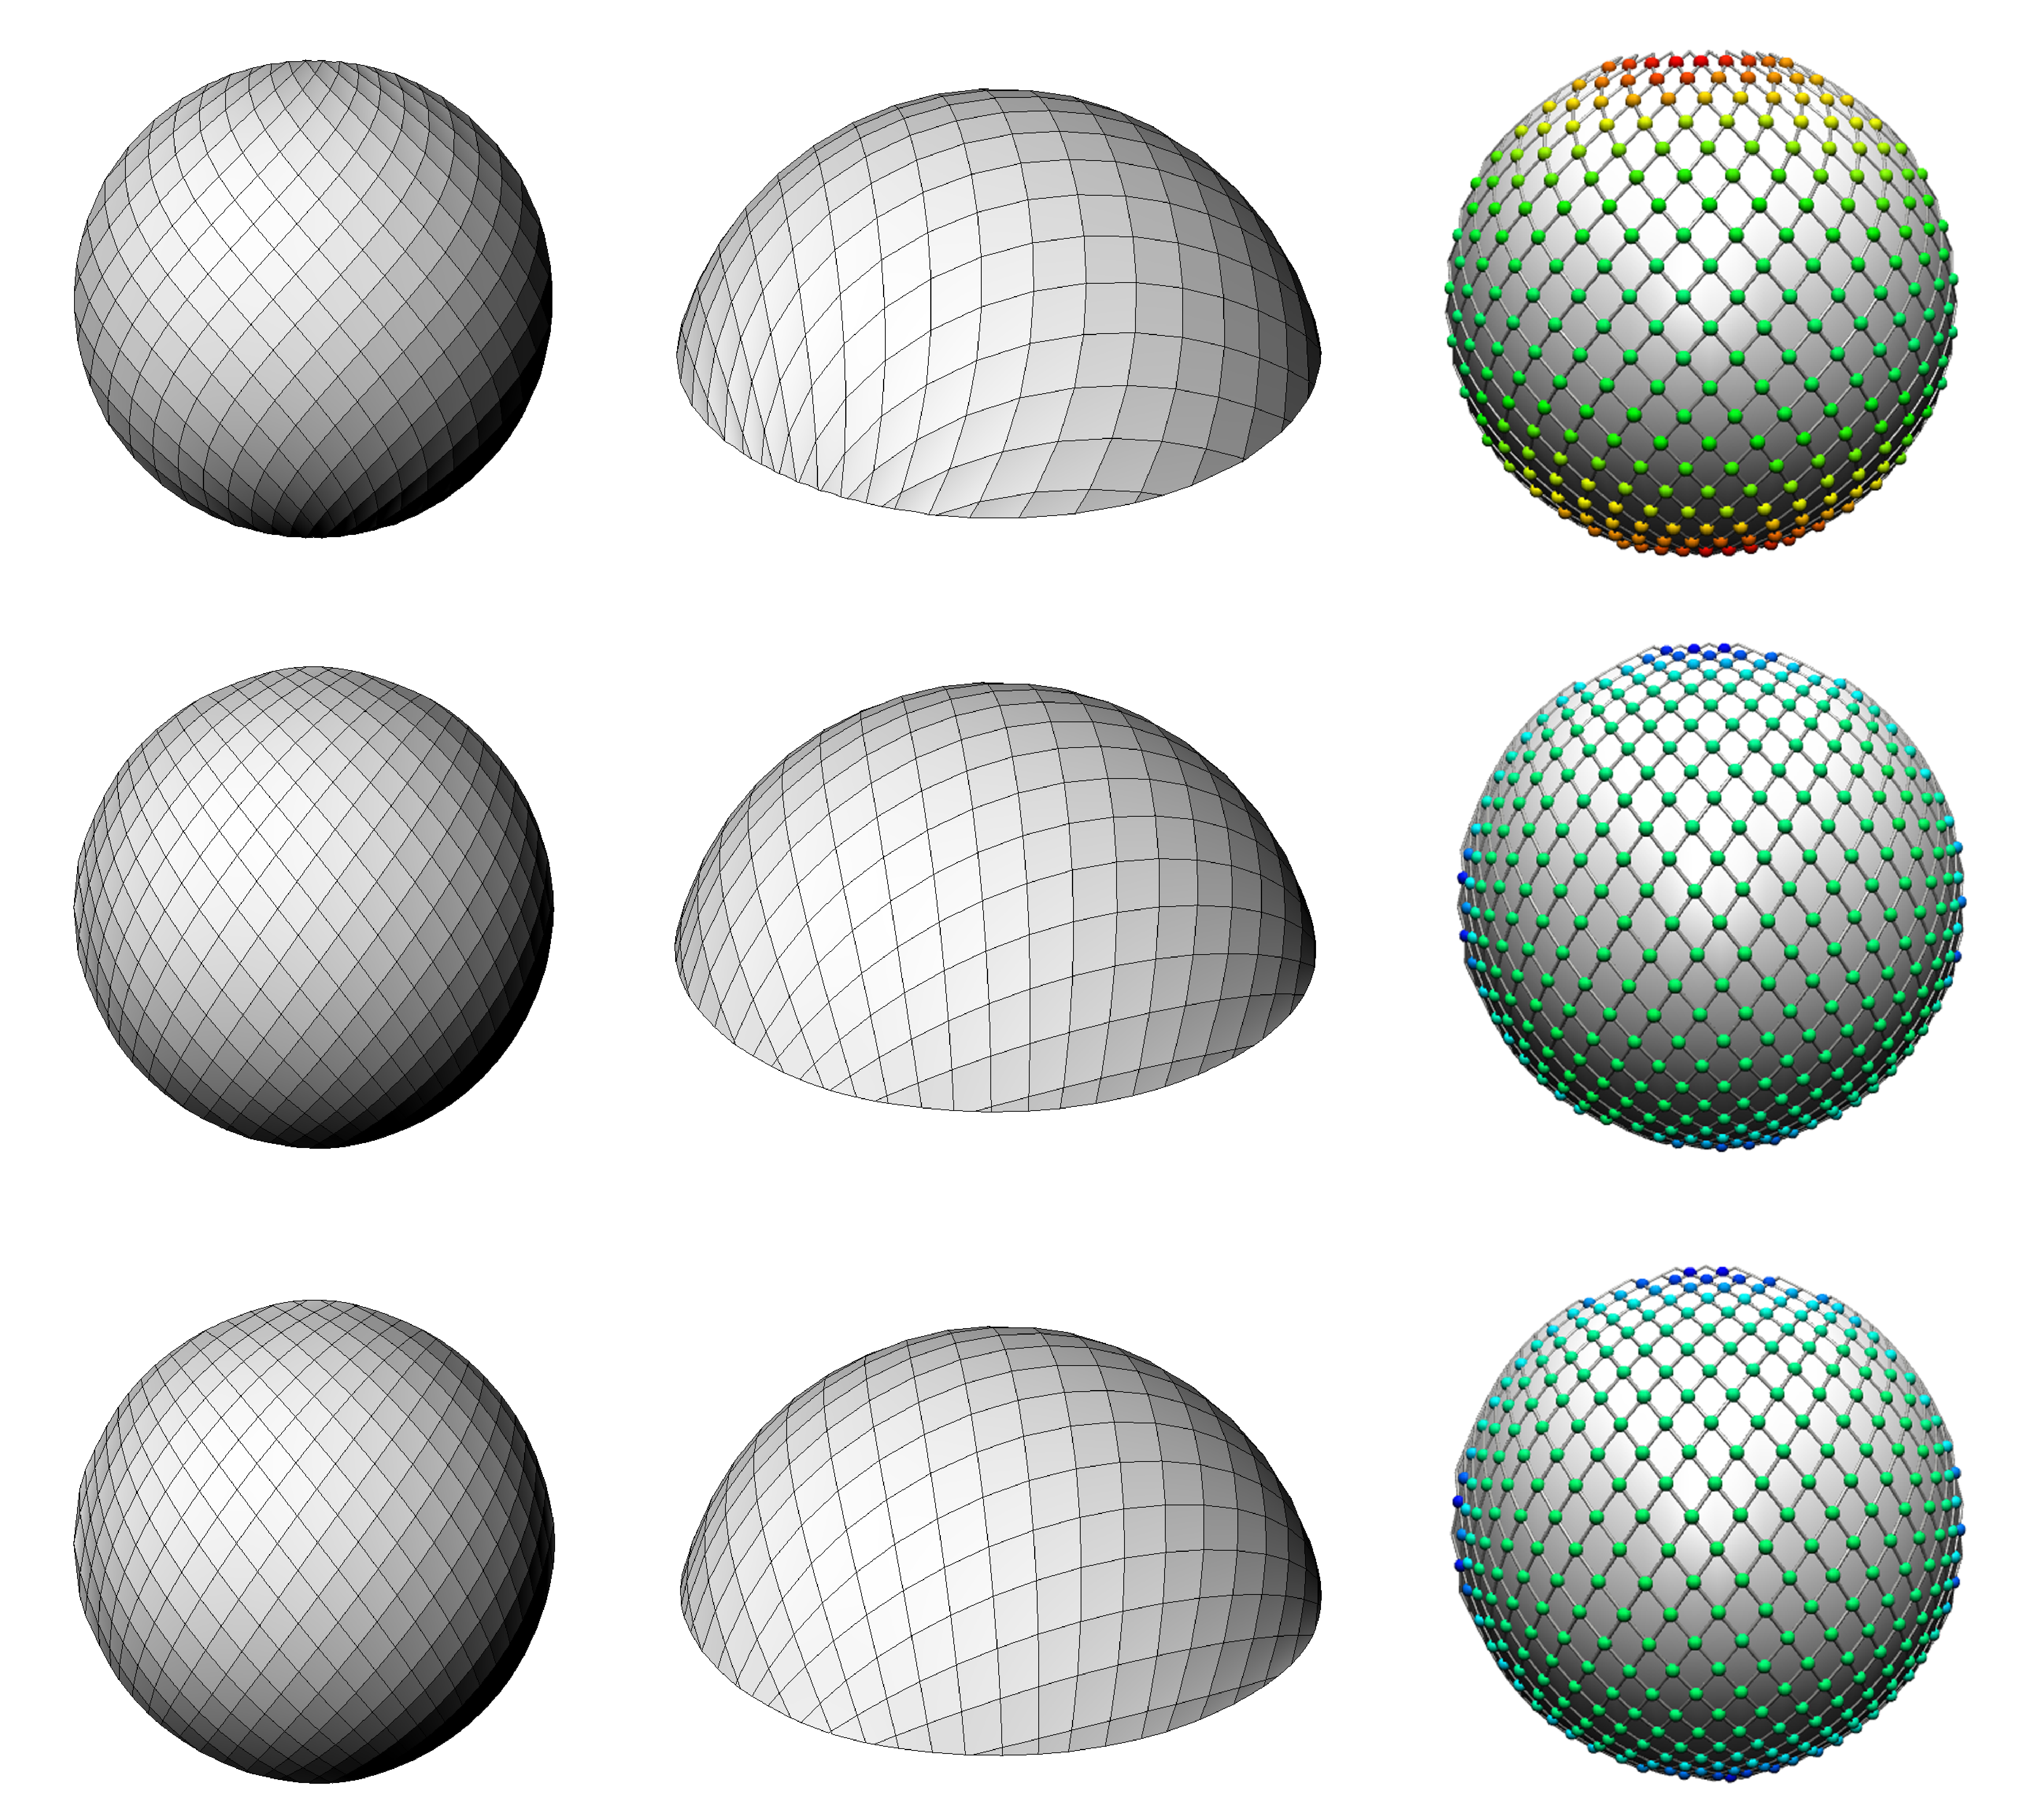
\includegraphics[width=0.80\linewidth]{images/CaseStudies_Irregular/SphereIrregular.pdf}
\caption{optimization of a spherical calotte with regular and irregular meshes. With a maximum variation of the segment length of 0.40m (middle) and 0.50m (bottom), the mean curvature of the grid could be reduced up to 83\% and 77\% respectively.}
\label{fig:SphereIrregular}
\end{figure}

\subsection{Practical application: The Flying Dome}

Elastic gridshells offer great advantages on temporary structures since the initially straight and afterwards elastically shaped profiles composing the grid allow rapid and cost-efficient production, transport and erection processes. For a temporary hanging 3D Projection Hemisphere (Flying Dome) of 10m diameter, an irregular elastic gridshell has been designed, see Figure~\ref{fig:Renderings}. The project is a cooperation between the UdK Berlin, the TU Berlin, the Fraunhofer Institut FIRST and industrial partners and is planned to be built in Berlin in October 2012.

The structure consists in a hybrid construction composed of an irregular elastic gridshell between a double-layer membrane stabilized by underpressure (vacuum) of 0.08mbar. The profiles of the gridshell are made of GFK and have a tubular section of 20mm diameter and 3mm thickness.A third layer of profiles assures the bracing of the grid and activates its shear-bearing capacity. A PVC-coated polyester fabric and a PVC projection foil have been planned for the outer and inner membranes, respectively. The extremities of the bent profiles are fixed on a steel box ring of 100x100x4mm. The hemisphere hangs from the roof through four cables of 6mm diameter and is horizontally stabilized by other four cables of 3mm diameter. The total weight of the structure is approximately 1.3 tons.

\begin{figure}
\centering
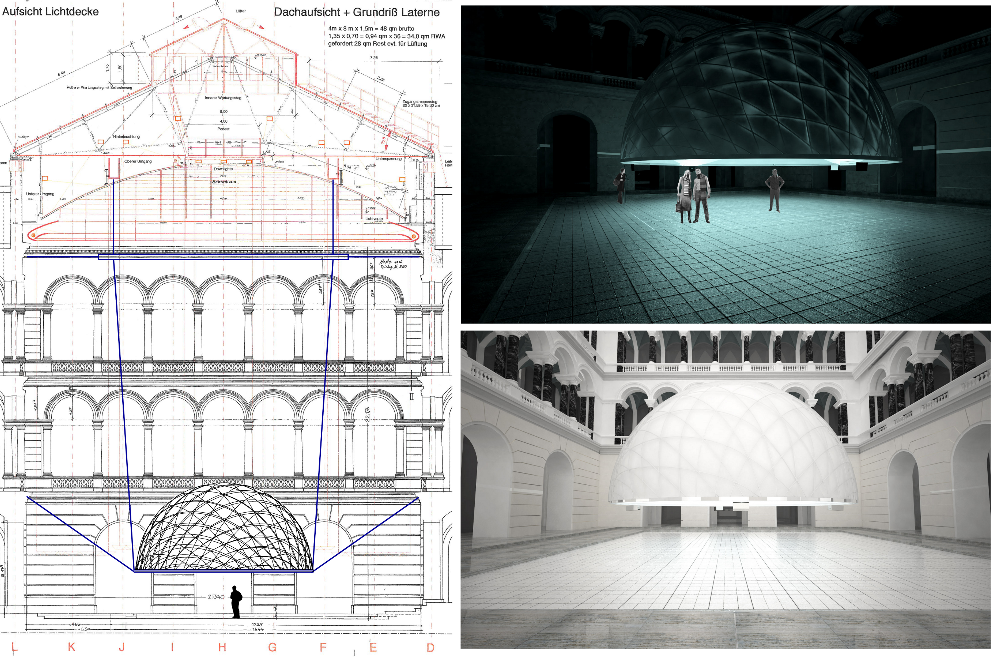
\includegraphics[width=1.0\linewidth]{images/Renderings_Modell/Renderings_lowres.pdf}
\caption{Front view and renderings of the Flying Dome}
\label{fig:Renderings}
\end{figure}

An irregular mesh was chosen in order to minimize the profiles curvature (the maximum curvature could be reduced up to 80\% compared to the regular gridshell) and to obtain a more interesting arrangement of the grid pattern. Physical modeling was used to analyze the visual effects, see Figure~\ref{fig:Modell}. 

\begin{figure}
\centering
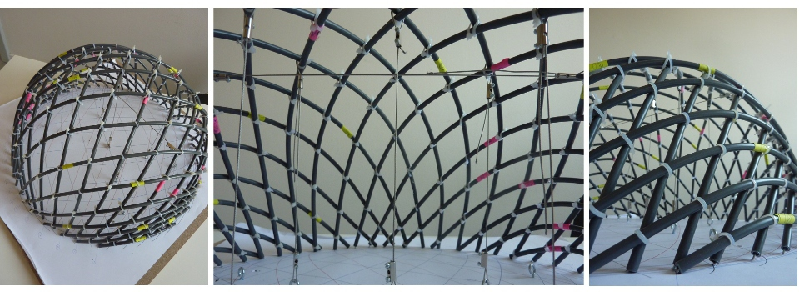
\includegraphics[width=1.0\linewidth]{images/Renderings_Modell/Modell.pdf}
\caption{Physical modeling of the Flying Dome to analyze the visual effects of the irregular mesh}
\label{fig:Modell}
\end{figure}

Contrary to regular grids, grids with irregular meshes cannot be completely deployed and can only be partially pre-assembled. The two profile layers will be joined and bent in a progressive process in order not to exceed the maximum allowable curvature during the erection of the structure. By means of finite element analysis, the assembling process of the hemisphere has been simulated and the maximum stresses during the shaping of the grid and by underpressure loading have been controlled, see Figure~\ref{fig:FEMGlobal}. 

\begin{figure}
\centering
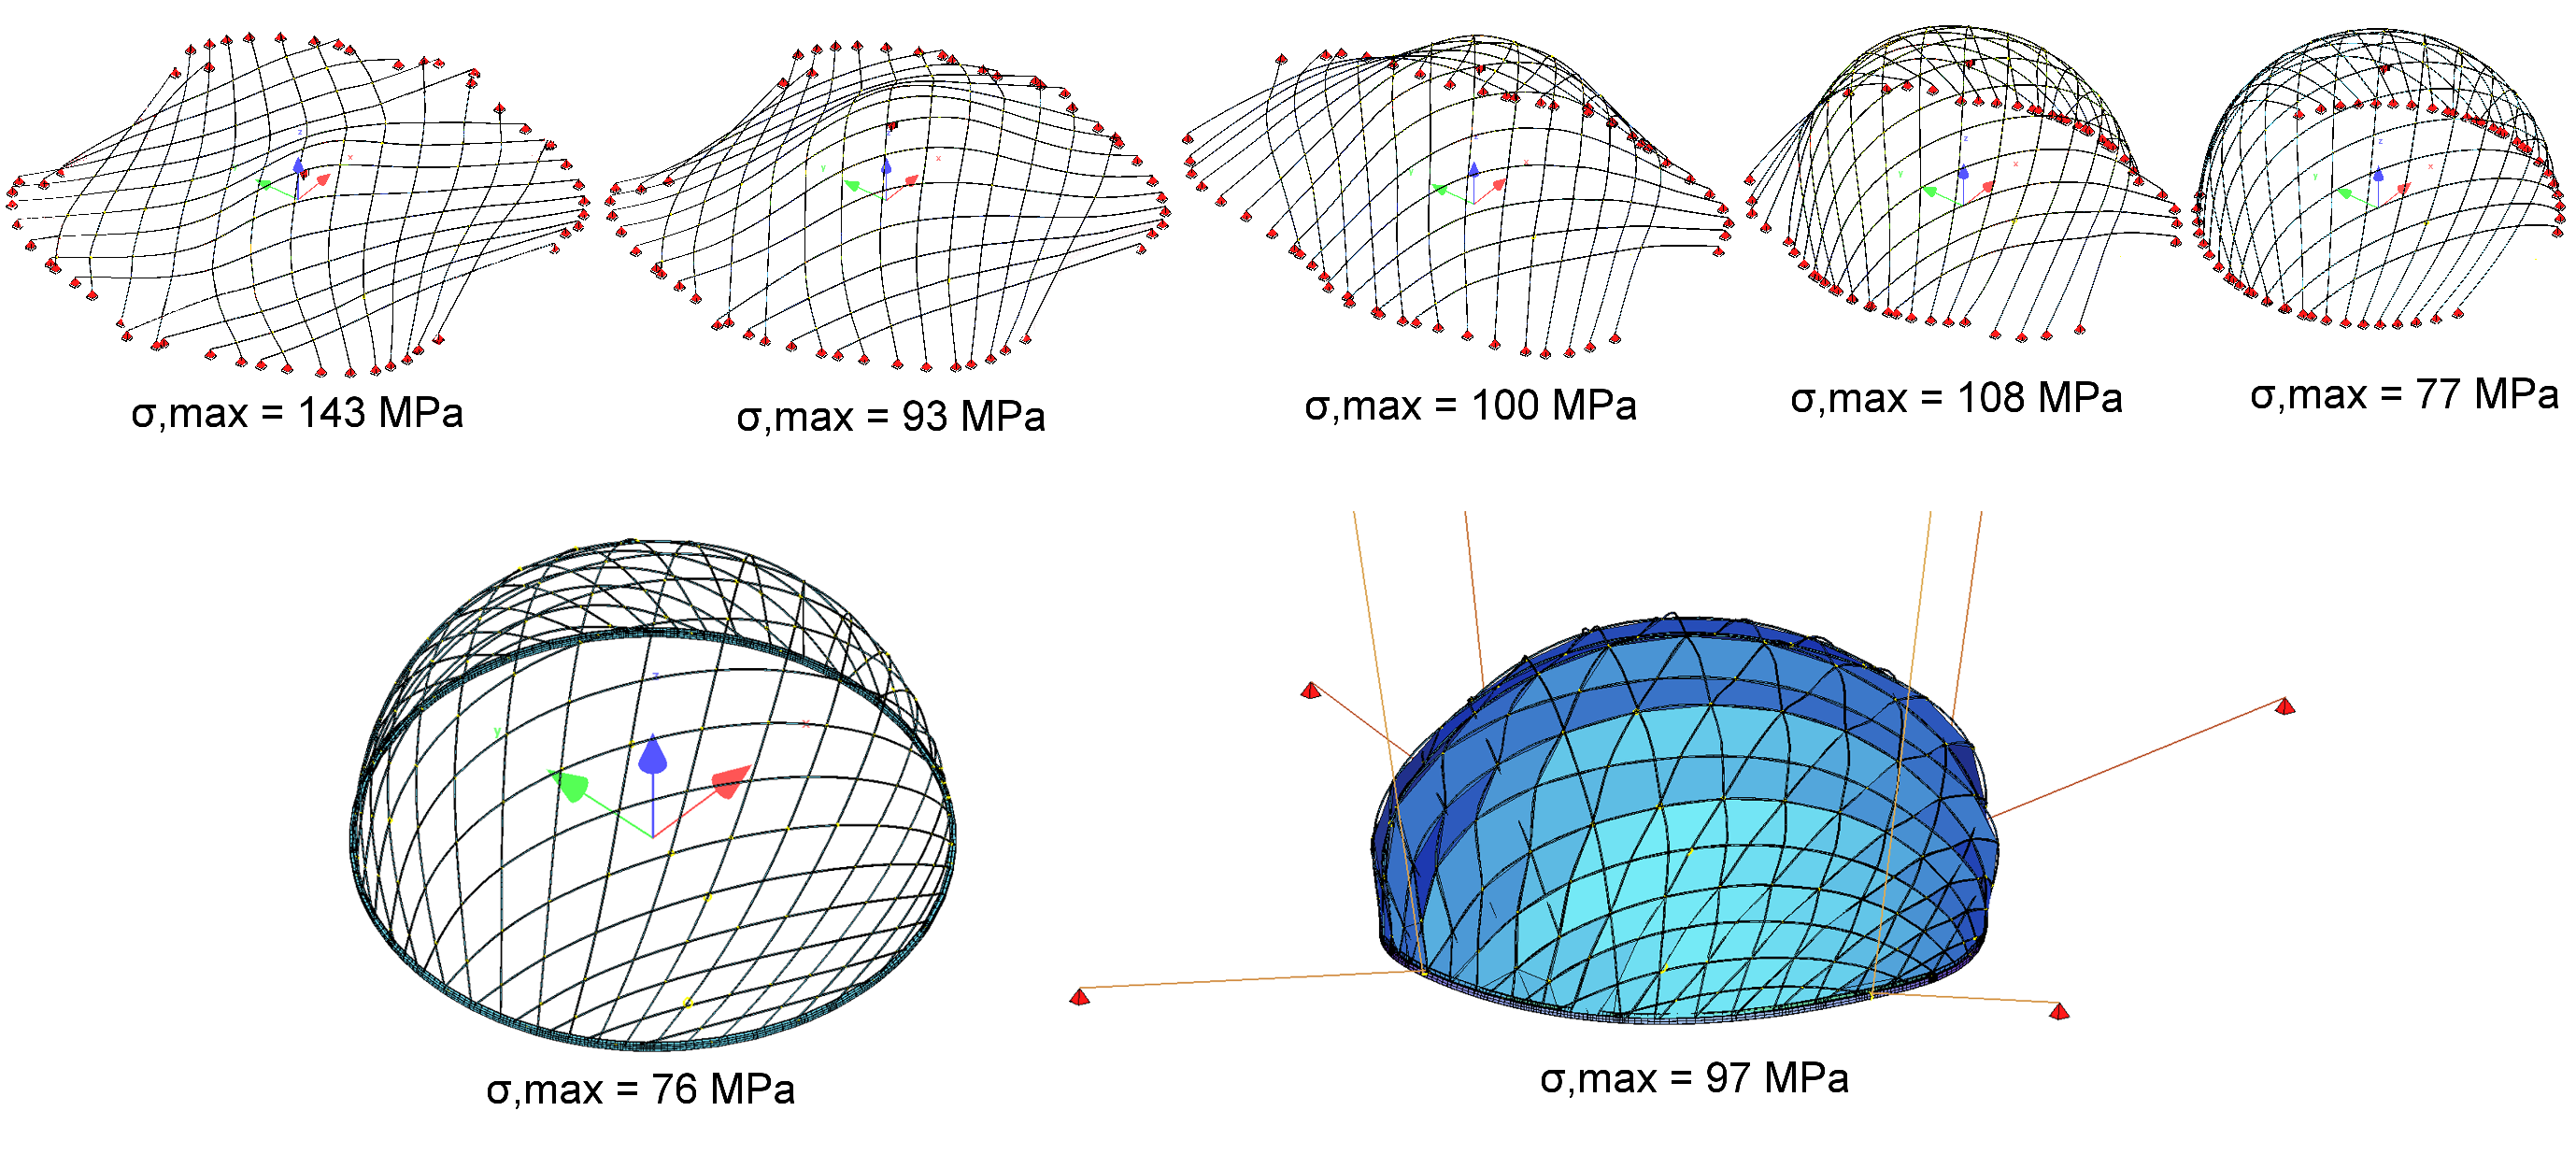
\includegraphics[width=1.0\linewidth]{images/CaseStudies_Irregular/FEMGlobal.pdf}
\caption{Simulation of the erection process and loading of the Flying Dome and analysis of the maximum stresses by means of FEA}
\label{fig:FEMGlobal}
\end{figure}


\section{Conclusion}

A non-linear variational method for optimizing topologies of regular and irregular elastic gridshells is presented in this paper. The design parameters {\it mesh size}, {\it reference surface} and {\it profiles curvature} are defined as penalizing energies with corresponding weighting factors. The resulting grid configuration is calculated by a non-linear algorithm by minimizing the linear combination of these three energies. The advantage of the variational method compared to other existing ones is that spacing between grid and target surface can be allowed and displacements of the grid nodes are possible in all directions, thus a further optimization of the grid topology can be achieved. Moreover, by defining different priorities between the design parameters through the energy weighting factors, diverse grid configurations can be generated and the resulting gridshell design can be adapted to specific structural and architectural requirements. 

%\section*{Acknowledgements}
%Stefan Sechelmann is supported by DFG Research Center \textsc{Matheon}, Thilo R\"orig by SFB/TR 109: Discretization in Geometry and Dynamics.
%We thank Andrew Furnas for pointing us to the Chebyshev parameterizations of the sphere by Voss. 

\subfilebibliography
\end{document}

%%% Local Variables:
%%% TeX-master: "Thesis.tex"
%%% End: